%  LaTeX support: latex@mdpi.com
%  For support, please attach all files needed for compiling as well as the log file, and specify your operating system, LaTeX version, and LaTeX editor.

%=================================================================
% pandoc conditionals added to preserve backwards compatibility with previous versions of rticles

\documentclass[notspecified,article,submit,moreauthors,pdftex]{Definitions/mdpi}


%% Some pieces required from the pandoc template
\setlist[itemize]{leftmargin=*,labelsep=5.8mm}
\setlist[enumerate]{leftmargin=*,labelsep=4.9mm}


%--------------------
% Class Options:
%--------------------

%---------
% article
%---------
% The default type of manuscript is "article", but can be replaced by:
% abstract, addendum, article, book, bookreview, briefreport, casereport, comment, commentary, communication, conferenceproceedings, correction, conferencereport, entry, expressionofconcern, extendedabstract, datadescriptor, editorial, essay, erratum, hypothesis, interestingimage, obituary, opinion, projectreport, reply, retraction, review, perspective, protocol, shortnote, studyprotocol, systematicreview, supfile, technicalnote, viewpoint, guidelines, registeredreport, tutorial
% supfile = supplementary materials

%----------
% submit
%----------
% The class option "submit" will be changed to "accept" by the Editorial Office when the paper is accepted. This will only make changes to the frontpage (e.g., the logo of the journal will get visible), the headings, and the copyright information. Also, line numbering will be removed. Journal info and pagination for accepted papers will also be assigned by the Editorial Office.

%------------------
% moreauthors
%------------------
% If there is only one author the class option oneauthor should be used. Otherwise use the class option moreauthors.

%---------
% pdftex
%---------
% The option pdftex is for use with pdfLaTeX. Remove "pdftex" for (1) compiling with LaTeX & dvi2pdf (if eps figures are used) or for (2) compiling with XeLaTeX.

%=================================================================
% MDPI internal commands - do not modify
\firstpage{1}
\makeatletter
\setcounter{page}{\@firstpage}
\makeatother
\pubvolume{1}
\issuenum{1}
\articlenumber{0}
\pubyear{2023}
\copyrightyear{2023}
%\externaleditor{Academic Editor: Firstname Lastname}
\datereceived{ }
\daterevised{ } % Comment out if no revised date
\dateaccepted{ }
\datepublished{ }
%\datecorrected{} % For corrected papers: "Corrected: XXX" date in the original paper.
%\dateretracted{} % For corrected papers: "Retracted: XXX" date in the original paper.
\hreflink{https://doi.org/} % If needed use \linebreak
%\doinum{}
%\pdfoutput=1 % Uncommented for upload to arXiv.org

%=================================================================
% Add packages and commands here. The following packages are loaded in our class file: fontenc, inputenc, calc, indentfirst, fancyhdr, graphicx, epstopdf, lastpage, ifthen, float, amsmath, amssymb, lineno, setspace, enumitem, mathpazo, booktabs, titlesec, etoolbox, tabto, xcolor, colortbl, soul, multirow, microtype, tikz, totcount, changepage, attrib, upgreek, array, tabularx, pbox, ragged2e, tocloft, marginnote, marginfix, enotez, amsthm, natbib, hyperref, cleveref, scrextend, url, geometry, newfloat, caption, draftwatermark, seqsplit
% cleveref: load \crefname definitions after \begin{document}

%=================================================================
% Please use the following mathematics environments: Theorem, Lemma, Corollary, Proposition, Characterization, Property, Problem, Example, ExamplesandDefinitions, Hypothesis, Remark, Definition, Notation, Assumption
%% For proofs, please use the proof environment (the amsthm package is loaded by the MDPI class).

%=================================================================
% Full title of the paper (Capitalized)
\Title{Full title of the paper (Capitalized)}

% MDPI internal command: Title for citation in the left column
\TitleCitation{Full title of the paper (Capitalized)}

% Author Orchid ID: enter ID or remove command
%\newcommand{\orcidauthorA}{0000-0000-0000-000X} % Add \orcidA{} behind the author's name
%\newcommand{\orcidauthorB}{0000-0000-0000-000X} % Add \orcidB{} behind the author's name


% Authors, for the paper (add full first names)
\Author{Dominik
Leutnant$^{1,2,\ddagger,*}$\href{https://orcid.org/0000-0003-3293-2315}
{\orcidicon}, John Doe$^{2, \dagger, \ddagger}$}


%\longauthorlist{yes}


% MDPI internal command: Authors, for metadata in PDF
\AuthorNames{Dominik Leutnant, John Doe}

% MDPI internal command: Authors, for citation in the left column
%\AuthorCitation{Lastname, F.; Lastname, F.; Lastname, F.}
% If this is a Chicago style journal: Lastname, Firstname, Firstname Lastname, and Firstname Lastname.
\AuthorCitation{Leutnant, D.; Doe, J.}

% Affiliations / Addresses (Add [1] after \address if there is only one affiliation.)
\address{%
$^{1}$ \quad Muenster University of Applied Sciences - Institute for
Infrastructure, Water, Resources, Environment Correnstr. 25, 48149
Muenster,
Germany; \href{mailto:leutnant@fh-muenster.de}{\nolinkurl{leutnant@fh-muenster.de}}\\
$^{2}$ \quad Your department Street, City,
Country; \href{mailto:mail@mail.com}{\nolinkurl{mail@mail.com}}\\
}

% Contact information of the corresponding author
\corres{Correspondence: \href{mailto:leutnant@fh-muenster.de}{\nolinkurl{leutnant@fh-muenster.de}};
Tel.: +XX-000-00-0000.}

% Current address and/or shared authorship
\firstnote{Current address: Updated affiliation}
\secondnote{These authors contributed equally to this work.}






% The commands \thirdnote{} till \eighthnote{} are available for further notes

% Simple summary
\simplesumm{A Simple summary goes here.}

%\conference{} % An extended version of a conference paper

% Abstract (Do not insert blank lines, i.e. \\)
\abstract{A single paragraph of about 200 words maximum. For research
articles, abstracts should give a pertinent overview of the work. We
strongly encourage authors to use the following style of structured
abstracts, but without headings: 1) Background: Place the question
addressed in a broad context and highlight the purpose of the study; 2)
Methods: Describe briefly the main methods or treatments applied; 3)
Results: Summarize the article's main findings; and 4) Conclusion:
Indicate the main conclusions or interpretations. The abstract should be
an objective representation of the article, it must not contain results
which are not presented and substantiated in the main text and should
not exaggerate the main conclusions.}


% Keywords
\keyword{keyword 1; keyword 2; keyword 3 (list three to ten pertinent
keywords specific to the article, yet reasonably common within the
subject discipline.).}

% The fields PACS, MSC, and JEL may be left empty or commented out if not applicable
%\PACS{J0101}
%\MSC{}
%\JEL{}

%%%%%%%%%%%%%%%%%%%%%%%%%%%%%%%%%%%%%%%%%%
% Only for the journal Diversity
%\LSID{\url{http://}}

%%%%%%%%%%%%%%%%%%%%%%%%%%%%%%%%%%%%%%%%%%
% Only for the journal Applied Sciences

%%%%%%%%%%%%%%%%%%%%%%%%%%%%%%%%%%%%%%%%%%

%%%%%%%%%%%%%%%%%%%%%%%%%%%%%%%%%%%%%%%%%%
% Only for the journal Data



%%%%%%%%%%%%%%%%%%%%%%%%%%%%%%%%%%%%%%%%%%
% Only for the journal Toxins


%%%%%%%%%%%%%%%%%%%%%%%%%%%%%%%%%%%%%%%%%%
% Only for the journal Encyclopedia


%%%%%%%%%%%%%%%%%%%%%%%%%%%%%%%%%%%%%%%%%%
% Only for the journal Advances in Respiratory Medicine
%\addhighlights{yes}
%\renewcommand{\addhighlights}{%

%\noindent This is an obligatory section in “Advances in Respiratory Medicine”, whose goal is to increase the discoverability and readability of the article via search engines and other scholars. Highlights should not be a copy of the abstract, but a simple text allowing the reader to quickly and simplified find out what the article is about and what can be cited from it. Each of these parts should be devoted up to 2~bullet points.\vspace{3pt}\\
%\textbf{What are the main findings?}
% \begin{itemize}[labelsep=2.5mm,topsep=-3pt]
% \item First bullet.
% \item Second bullet.
% \end{itemize}\vspace{3pt}
%\textbf{What is the implication of the main finding?}
% \begin{itemize}[labelsep=2.5mm,topsep=-3pt]
% \item First bullet.
% \item Second bullet.
% \end{itemize}
%}


%%%%%%%%%%%%%%%%%%%%%%%%%%%%%%%%%%%%%%%%%%

% Pandoc syntax highlighting
\usepackage{color}
\usepackage{fancyvrb}
\newcommand{\VerbBar}{|}
\newcommand{\VERB}{\Verb[commandchars=\\\{\}]}
\DefineVerbatimEnvironment{Highlighting}{Verbatim}{commandchars=\\\{\}}
% Add ',fontsize=\small' for more characters per line
\usepackage{framed}
\definecolor{shadecolor}{RGB}{248,248,248}
\newenvironment{Shaded}{\begin{snugshade}}{\end{snugshade}}
\newcommand{\AlertTok}[1]{\textcolor[rgb]{0.94,0.16,0.16}{#1}}
\newcommand{\AnnotationTok}[1]{\textcolor[rgb]{0.56,0.35,0.01}{\textbf{\textit{#1}}}}
\newcommand{\AttributeTok}[1]{\textcolor[rgb]{0.13,0.29,0.53}{#1}}
\newcommand{\BaseNTok}[1]{\textcolor[rgb]{0.00,0.00,0.81}{#1}}
\newcommand{\BuiltInTok}[1]{#1}
\newcommand{\CharTok}[1]{\textcolor[rgb]{0.31,0.60,0.02}{#1}}
\newcommand{\CommentTok}[1]{\textcolor[rgb]{0.56,0.35,0.01}{\textit{#1}}}
\newcommand{\CommentVarTok}[1]{\textcolor[rgb]{0.56,0.35,0.01}{\textbf{\textit{#1}}}}
\newcommand{\ConstantTok}[1]{\textcolor[rgb]{0.56,0.35,0.01}{#1}}
\newcommand{\ControlFlowTok}[1]{\textcolor[rgb]{0.13,0.29,0.53}{\textbf{#1}}}
\newcommand{\DataTypeTok}[1]{\textcolor[rgb]{0.13,0.29,0.53}{#1}}
\newcommand{\DecValTok}[1]{\textcolor[rgb]{0.00,0.00,0.81}{#1}}
\newcommand{\DocumentationTok}[1]{\textcolor[rgb]{0.56,0.35,0.01}{\textbf{\textit{#1}}}}
\newcommand{\ErrorTok}[1]{\textcolor[rgb]{0.64,0.00,0.00}{\textbf{#1}}}
\newcommand{\ExtensionTok}[1]{#1}
\newcommand{\FloatTok}[1]{\textcolor[rgb]{0.00,0.00,0.81}{#1}}
\newcommand{\FunctionTok}[1]{\textcolor[rgb]{0.13,0.29,0.53}{\textbf{#1}}}
\newcommand{\ImportTok}[1]{#1}
\newcommand{\InformationTok}[1]{\textcolor[rgb]{0.56,0.35,0.01}{\textbf{\textit{#1}}}}
\newcommand{\KeywordTok}[1]{\textcolor[rgb]{0.13,0.29,0.53}{\textbf{#1}}}
\newcommand{\NormalTok}[1]{#1}
\newcommand{\OperatorTok}[1]{\textcolor[rgb]{0.81,0.36,0.00}{\textbf{#1}}}
\newcommand{\OtherTok}[1]{\textcolor[rgb]{0.56,0.35,0.01}{#1}}
\newcommand{\PreprocessorTok}[1]{\textcolor[rgb]{0.56,0.35,0.01}{\textit{#1}}}
\newcommand{\RegionMarkerTok}[1]{#1}
\newcommand{\SpecialCharTok}[1]{\textcolor[rgb]{0.81,0.36,0.00}{\textbf{#1}}}
\newcommand{\SpecialStringTok}[1]{\textcolor[rgb]{0.31,0.60,0.02}{#1}}
\newcommand{\StringTok}[1]{\textcolor[rgb]{0.31,0.60,0.02}{#1}}
\newcommand{\VariableTok}[1]{\textcolor[rgb]{0.00,0.00,0.00}{#1}}
\newcommand{\VerbatimStringTok}[1]{\textcolor[rgb]{0.31,0.60,0.02}{#1}}
\newcommand{\WarningTok}[1]{\textcolor[rgb]{0.56,0.35,0.01}{\textbf{\textit{#1}}}}

% tightlist command for lists without linebreak
\providecommand{\tightlist}{%
  \setlength{\itemsep}{0pt}\setlength{\parskip}{0pt}}



\makeatletter
\providecommand{\pandocbounded}[1]{#1}
\makeatother
\usepackage{longtable}

\begin{document}



%%%%%%%%%%%%%%%%%%%%%%%%%%%%%%%%%%%%%%%%%%

\section{Version}\label{version}

This Rmd-skeleton uses the mdpi Latex template published 2023-03-25.
However, the official template gets more frequently updated than the
\textbf{rticles} package. Therefore, please make sure prior to paper
submission, that you're using the most recent .cls, .tex and .bst files
(available \href{http://www.mdpi.com/authors/latex}{here}).

\section{Article Header Information}\label{article-header-information}

The YAML header includes information needed mainly for formatting the
front and back matter of the article. Required elements include:

\begin{Shaded}
\begin{Highlighting}[]
\FunctionTok{title}\KeywordTok{:}\AttributeTok{ Title of the paper}
\FunctionTok{author}\KeywordTok{:}
\AttributeTok{  }\KeywordTok{{-}}\AttributeTok{ }\FunctionTok{name}\KeywordTok{:}\AttributeTok{ first and last name}
\FunctionTok{    affil}\KeywordTok{: }\CharTok{|}
\NormalTok{      One or more comma seperated numbers corresponding to affilitation}
\NormalTok{      and one or more  comma seperated symbols corresponding }
\NormalTok{      optional notes.}
\AttributeTok{    }\FunctionTok{orcid}\KeywordTok{:}\AttributeTok{ optional orcid number}
\FunctionTok{affiliation}\KeywordTok{:}\AttributeTok{  }
\AttributeTok{  }\KeywordTok{{-}}\AttributeTok{ }\FunctionTok{num}\KeywordTok{:}\AttributeTok{ 1,..., n for each affiliation}
\AttributeTok{    }\FunctionTok{address}\KeywordTok{:}\AttributeTok{ required}
\AttributeTok{    }\FunctionTok{email}\KeywordTok{:}\AttributeTok{ required}
\FunctionTok{authorcitation}\KeywordTok{: }\CharTok{|}
\NormalTok{  Lastname, F.}
\FunctionTok{correspondence}\KeywordTok{: }\CharTok{|}
\NormalTok{  email@email.com; Tel.: +XX{-}000{-}00{-}0000.}
\FunctionTok{journal}\KeywordTok{:}\AttributeTok{ notspecified}
\FunctionTok{type}\KeywordTok{:}\AttributeTok{ article}
\FunctionTok{status}\KeywordTok{:}\AttributeTok{ submit}
\end{Highlighting}
\end{Shaded}

Journal options are in Table \ref{tab:mdpinames}. The \texttt{status}
variable should generally not be changed by authors. The \texttt{type}
variable describes the type of of submission and defaults to
\texttt{article} but can be replaced with any of the ones in Table
\ref{tab:mdpitype}

\begin{table}

\caption{\label{tab:mdpitype}MDPI article types.}
\centering
\begin{tabular}[t]{lll}
\toprule
abstract & entry & retraction\\
addendum & expressionofconcern & review\\
article & extendedabstract & perspective\\
book & datadescriptor & protocol\\
bookreview & editorial & shortnote\\
\addlinespace
briefreport & essay & studyprotocol\\
casereport & erratum & systematicreview\\
comment & hypothesis & supfile\\
commentary & interestingimage & technicalnote\\
communication & obituary & viewpoint\\
\addlinespace
conferenceproceedings & opinion & guidelines\\
correction & projectreport & registeredreport\\
conferencereport & reply & tutorial\\
\bottomrule
\end{tabular}
\end{table}

\subsection{Journal Specific YAML
variables}\label{journal-specific-yaml-variables}

\begin{Shaded}
\begin{Highlighting}[]
\CommentTok{\# for journal Diversity,}
\CommentTok{\# add the Life Science Identifier using:}
\FunctionTok{lsid}\KeywordTok{:}\AttributeTok{ http://zoobank.org/urn:lsid:zoobank.org:act:nnnn}


\CommentTok{\# for journal Applied Sciences}
\CommentTok{\# add featured application}
\FunctionTok{featuredapplication}\KeywordTok{: }\CharTok{|}
\NormalTok{  Authors are encouraged to provide a concise }
\NormalTok{  description of the specific application or }
\NormalTok{  a potential application of the work. This }
\NormalTok{  section is not mandatory.}

\CommentTok{\# for the journal Data}
\CommentTok{\# add dataset doi and license}
\FunctionTok{dataset}\KeywordTok{:}\AttributeTok{ https://doi.org/10.1000/182}
\FunctionTok{datasetlicense}\KeywordTok{:}\AttributeTok{ CC{-}BY{-}4.0}

\CommentTok{\# for the journal Toxins}
\CommentTok{\# add key contributions}
\FunctionTok{keycontributions}\KeywordTok{: }\CharTok{|}
\NormalTok{  The breakthroughs or highlights of the manuscript. }
\NormalTok{  Authors can write one or two sentences to describe }
\NormalTok{  the most important part of the paper.}

\CommentTok{\# for the journal Encyclopedia}
\FunctionTok{encyclopediadef}\KeywordTok{: }\CharTok{|}
\NormalTok{  For entry manuscripts only: please provide a brief overview}
\NormalTok{  of the entry title instead of an abstract.}
\FunctionTok{entrylink}\KeywordTok{:}\AttributeTok{ The Link to this entry published on the encyclopedia platform.}

\CommentTok{\# for the journal Advances in Respiratory Medicine}
\CommentTok{\# add highlights}
\FunctionTok{addhighlights}\KeywordTok{: }\CharTok{|}
\NormalTok{  This is an obligatory section in “Advances in Respiratory Medicine”, }
\NormalTok{  whose goal is to increase the discoverability and readability of the}
\NormalTok{  article via search engines and other scholars. Highlights should not }
\NormalTok{  be a copy of the abstract, but a simple text allowing the reader to }
\NormalTok{  quickly and simplified find out what the article is about and what can }
\NormalTok{  be cited from it. Each of these parts should be devoted up to 2\textasciitilde{}bullet }
\NormalTok{  points.}
\end{Highlighting}
\end{Shaded}

\startlandscape

\begin{longtable}[t]{llllllll}
\caption{\label{tab:mdpinames}MDPI journal names.}\\
\toprule
acoustics & biomedinformatics & dentistry & galaxies & jcp & metabolites & philosophies & socsci\\
actuators & biomimetics & dermato & games & jcs & metals & photochem & software\\
addictions & biomolecules & dermatopathology & gases & jcto & meteorology & photonics & soilsystems\\
admsci & biophysica & designs & gastroent & jdb & methane & phycology & solar\\
adolescents & biosensors & devices & gastrointestdisord & jeta & metrology & physchem & solids\\
\addlinespace
aerobiology & biotech & diabetology & gels & jfb & micro & physics & spectroscj\\
aerospace & birds & diagnostics & genealogy & jfmk & microarrays & physiologia & sports\\
agriculture & bloods & dietetics & genes & jimaging & microbiolres & plants & standards\\
agriengineering & blsf & digital & geographies & jintelligence & micromachines & plasma & stats\\
agrochemicals & brainsci & disabilities & geohazards & jlpea & microorganisms & platforms & std\\
\addlinespace
agronomy & breath & diseases & geomatics & jmmp & microplastics & pollutants & stresses\\
ai & buildings & diversity & geosciences & jmp & minerals & polymers & surfaces\\
air & businesses & dna & geotechnics & jmse & mining & polysaccharides & surgeries\\
algorithms & cancers & drones & geriatrics & jne & modelling & poultry & suschem\\
allergies & carbon & dynamics & grasses & jnt & molbank & powders & sustainability\\
\addlinespace
alloys & cardiogenetics & earth & gucdd & jof & molecules & preprints & symmetry\\
analytica & catalysts & ebj & hazardousmatters & joitmc & mps & proceedings & synbio\\
analytics & cells & ecologies & healthcare & jor & msf & processes & systems\\
anatomia & ceramics & econometrics & hearts & journalmedia & mti & prosthesis & targets\\
animals & challenges & economies & hemato & jox & muscles & proteomes & taxonomy\\
\addlinespace
antibiotics & chemengineering & education & hematolrep & jpm & nanoenergyadv & psf & technologies\\
antibodies & chemistry & ejihpe & heritage & jrfm & nanomanufacturing & psych & telecom\\
antioxidants & chemosensors & electricity & higheredu & jsan & nanomaterials & psychiatryint & test\\
applbiosci & chemproc & electrochem & highthroughput & jtaer & ncrna & psychoactives & textiles\\
appliedchem & children & electronicmat & histories & jvd & ndt & publications & thalassrep\\
\addlinespace
appliedmath & chips & electronics & horticulturae & jzbg & network & quantumrep & thermo\\
applmech & cimb & encyclopedia & hospitals & kidneydial & neuroglia & quaternary & tomography\\
applmicrobiol & civileng & endocrines & humanities & kinasesphosphatases & neurolint & qubs & tourismhosp\\
applnano & cleantechnol & energies & humans & knowledge & neurosci & radiation & toxics\\
applsci & climate & eng & hydrobiology & land & nitrogen & reactions & toxins\\
\addlinespace
aquacj & clinpract & engproc & hydrogen & languages & notspecified & receptors & transplantology\\
architecture & clockssleep & entomology & hydrology & laws & nri & recycling & transportation\\
arm & cmd & entropy & hygiene & life & nursrep & regeneration & traumacare\\
arthropoda & coasts & environments & idr & liquids & nutraceuticals & religions & traumas\\
arts & coatings & environsciproc & ijerph & literature & nutrients & remotesensing & tropicalmed\\
\addlinespace
asc & colloids & epidemiologia & ijfs & livers & obesities & reports & universe\\
asi & colorants & epigenomes & ijgi & logics & oceans & reprodmed & urbansci\\
astronomy & commodities & est & ijms & logistics & ohbm & resources & uro\\
atmosphere & compounds & fermentation & ijns & lubricants & onco & rheumato & vaccines\\
atoms & computation & fibers & ijpb & lymphatics & oncopathology & risks & vehicles\\
\addlinespace
audiolres & computers & fintech & ijtm & machines & optics & robotics & venereology\\
automation & condensedmatter & fire & ijtpp & macromol & oral & ruminants & vetsci\\
axioms & conservation & fishes & ime & magnetism & organics & safety & vibration\\
bacteria & constrmater & fluids & immuno & magnetochemistry & organoids & sci & virtualworlds\\
batteries & cosmetics & foods & informatics & make & osteology & scipharm & viruses\\
\addlinespace
bdcc & covid & forecasting & information & marinedrugs & oxygen & sclerosis & vision\\
behavsci & crops & forensicsci & infrastructures & materials & parasites & seeds & waste\\
beverages & cryptography & forests & inorganics & materproc & parasitologia & sensors & water\\
biochem & crystals & foundations & insects & mathematics & particles & separations & wem\\
bioengineering & csmf & fractalfract & instruments & mca & pathogens & sexes & wevj\\
\addlinespace
biologics & ctn & fuels & inventions & measurements & pathophysiology & signals & wind\\
biology & curroncol & future & iot & medicina & pediatrrep & sinusitis & women\\
biomass & cyber & futureinternet & j & medicines & pharmaceuticals & skins & world\\
biomechanics & dairy & futurepharmacol & jal & medsci & pharmaceutics & smartcities & youth\\
biomed & data & futurephys & jcdd & membranes & pharmacoepidemiology & sna & zoonoticdis\\
\addlinespace
biomedicines & ddc & futuretransp & jcm & merits & pharmacy & societies & \\
\bottomrule
\end{longtable}
\finishlandscape

\section{Introducción}\label{introducciuxf3n}

Aquí escribiremos la introducción del trabajo

PREGUNTA CLAVE: ¿Existe una correspondencia real entre las prioridades
de gasto de los gobiernos y las necesidades epidemiológicas de su
población?

\section{Materiales y Métodos}\label{materiales-y-muxe9todos}

\begin{verbatim}
## 
## Adjuntando el paquete: 'dplyr'
\end{verbatim}

\begin{verbatim}
## The following objects are masked from 'package:stats':
## 
##     filter, lag
\end{verbatim}

\begin{verbatim}
## The following objects are masked from 'package:base':
## 
##     intersect, setdiff, setequal, union
\end{verbatim}

\subsection{Fuente y obtención de los
datos}\label{fuente-y-obtenciuxf3n-de-los-datos}

Los datos utilizados en este trabajo proceden del Banco Mundial,
concretamente de la base de datos \emph{World Development Indicators}
(WDI). Esta base de datos recopila indicadores tanto económicos como
sanitarios o demográficos de países de todo el mundo, lo que nos
permitirá realizar comparaciones internacionales.

La obtención de los datos se ha realizado mendiante el paquete WDI de R,
que permite acceder y descargar directamente los datos del Banco
Mundial. Esta base de datos contiene indicadores económicos, sociales y
demográficos a nivel mundial, con datos para aproximadamente 200 países
y sus regiones desde 1960.

Teniendo en cuenta las preguntas que se han formulado inicialmente, se
ha elegido un subconjunto de variables de interés, para formar un
dataset propio. Estas variables son:

\begin{itemize}
\item
  \textbf{Esperanza de vida al nacer (total)}: número de años que un
  recién nacido viviría si los patrones de mortalidad del momento se
  mantienen a lo largo de vida (años). \emph{Código: SP.DYN.LE00.IN.}
\item
  \textbf{PIB per capita}: Producto Interior Bruto, ganancias totales
  ganadas mediante la producción de bienes y servicioes en un territorio
  económico durante un periodo contable, y dividido entre la población
  general (US\$).\emph{Código: NY.GDP.PCAP.CD.}
\item
  \textbf{Gasto en salud}: Estimación de los gastos en salud icluyendo
  los productos y servicios sanitarios consumidos cada año, sin incluir
  edificios, maquinaria, IT y stocks de vacunas para emergencias (\%
  PIB). \emph{Código: SH.XPD.CHEX.GD.ZS.}
\item
  \textbf{Gasto en defensa}: Gasto en defensa respecto al PIB (\% PIB).
  \emph{Código: MS.MIL.XPND.GD.ZS.}
\item
  \textbf{Mortalidad infantil}: Número de muertes de bebes de 0 a 12
  meses por cada 1000 nacimientos al año (n:1000). \emph{Código:
  SP.DYN.IMRT.IN}.
\item
  \textbf{Acceso al agua}: Personas utilizando los servicios mínimos
  básicos de agua potable (\% población). \emph{Código: SH.H2O.BASW.ZS.}
\item
  \textbf{Escolaridad secundaria (total)}: Niños que reciben educación
  secundaria básica oficial (\% neto). \emph{Código: SE.SEC.NENR.}
\item
  \textbf{Causa de muerte por enf. agudas}: Personas que han fallecido
  por enfermedades agudas, que incluyen enfermedades infecciosas y
  parasitarias, infecciones respiratorias y deficiencias nutricionales
  (\% del total de muertes). \emph{Código: SH.DTH.COMM.ZS}.
\item
  \textbf{Causa de muerte por enf. crónicas}: Personas que han fallecido
  por enfermedades crónicas, que incluyen cáncer, diabetes, trastonos
  cardiovasculares, digestivos, dermatológicos, musculoesqueléticos y
  anomalías congenitales (\% del total de muertes). \emph{Código:
  SH.DTH.NCOM.ZS.}
\item
  \textbf{Mortalidad por falta de higiene}: Personas que han muerto por
  el uso de agua en malas condiciones, condiciones sanitarias inseguras
  y falta de higiene (número de muertes por 100.000 personas).
  \emph{Código: SH.STA.WASH.P5.}
\item
  \textbf{Fertilidad}: Número de niños que daría a luz una mujer si
  viviese hasta el final de sus años fértiles en el momento temporal
  captado (nacimientos por mujer). \emph{Código: SP.DYN.TFRT.IN.}
\item
  \textbf{Embarazos adolescentes}: Ratio de fertilidad adolescente,
  número de nacimientos por cada 1000 mujeres con una edad entre 15 y 19
  años (nacimientos por 1000 adolescentes). \emph{Código: SP.ADO.TFRT}.
  YE
\item
  \textbf{Población}: Número de residentes del país estimados a mitad
  del año (\#personas). \emph{Código: SP.POP.TOTL.}
\item
  \textbf{Area}: Superfície total del país potencialmente habitable,
  excluyendo el área ocupada por agua (ríos y lagos), y zonas
  exclusivamente económicas/laborales (\(km^2\)). \emph{Código:
  AG.LND.TOTL.K2.}
\item
  \textbf{Mortalidad por contaminación del aire}: Número de muertes por
  transtornos derivados de la inhalación de partículas contaminantes
  presentes en el aire (muertes por 100.000 habitantes). \emph{Código:
  CC.SH.AIRP.AMB.}
\item
  \textbf{Inmunización}: Número de niños inmunizados completamente entre
  15 y 23 meses (\%). \emph{Código: HF.IMM.FULL.}
\end{itemize}

De todo el registro de años con los que se cuenta en el dataset del
Banco Mundial, se tomaron datos del 2015 al 2022 para acotar el análisis
en la primera fase de exploración inicial de los datos, puesto que son
los años más recientes y de los que potencialmente se cuente con más
cantidad de datos actualizados.

\subsection{Selección de la muestra}\label{selecciuxf3n-de-la-muestra}

Dado que los datos descargados eran extremadamente abundantes (2476
observaciones de 29 variables), con `3 dimensiones' (temporal, indicador
y países), se realizó una exploración inicial de los datos descargados
para elegir un año y descartar las variables con un porcentaje de datos
faltantes superior al 70\%.

Tras este análisis exploratorio (documento
\texttt{Exploración\_inicial.Rmd}), se tomó la cohorte de 218 países del
año 2019, con 17 variables: el país, clasificación de `income', región,
año, esperanza de vida, fertilidad, embarazos adolescentes, población,
PIB por capita, gasto en salud, gasto en defensa, mortalidad infantil,
acceso a agua, mortalidad por enf. agudas, mortalidad por enf. crónicas,
mortalidad por falta de higiene y densidad demográfica (una variable
adicional creada a partir de la población y el área del país). El resto
de variables fueron descartadas.

\section{Resultados}\label{resultados}

A continuación se muestran los resultados del estudio, divididos en 4
bloques, que están organizados de modo que permitan responder a la
pregunta principal del trabajo.

\begin{itemize}
\item
  Bloque 1. \textbf{Contexto socioeconómico de los países}.
\item
  Bloque 2. \textbf{Comparación del gasto en salud y en defensa de los
  países}.
\item
  Bloque 3. \textbf{Necesidades sanitarias por países}.
\item
  Bloque 4. \textbf{Agregación final: correspondencia entre el gasto
  público y las necesidades de los ciudadanos del país}.
\end{itemize}

\subsection{Bloque 1. Contexto
socioeconómico.}\label{bloque-1.-contexto-socioeconuxf3mico.}

El objetivo es analizar el PIB por cápita de los diferentes países,
agrupándolos atendiendo a la variable `income'. Asimismo, se estudiará a
las regiones a las que pertenece cada país, por grupos, para determinar
si existe alguna relación entre situación económica y localización
geográfica. Finalmente, se incorporará el concepto de densidad
demográfica para estudiar si existe una relación entre esta y el PIB por
cápita del país.

\pandocbounded{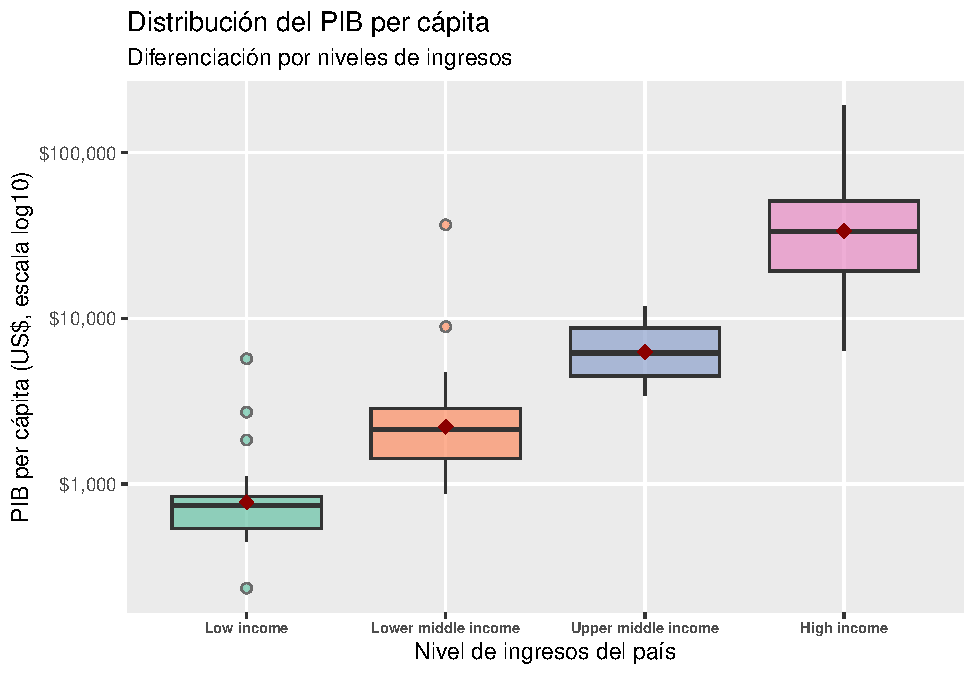
\includegraphics[keepaspectratio]{Untitled_files/figure-latex/unnamed-chunk-2-1.pdf}}

\begin{verbatim}
## Saving 6.5 x 4.5 in image
\end{verbatim}

\pandocbounded{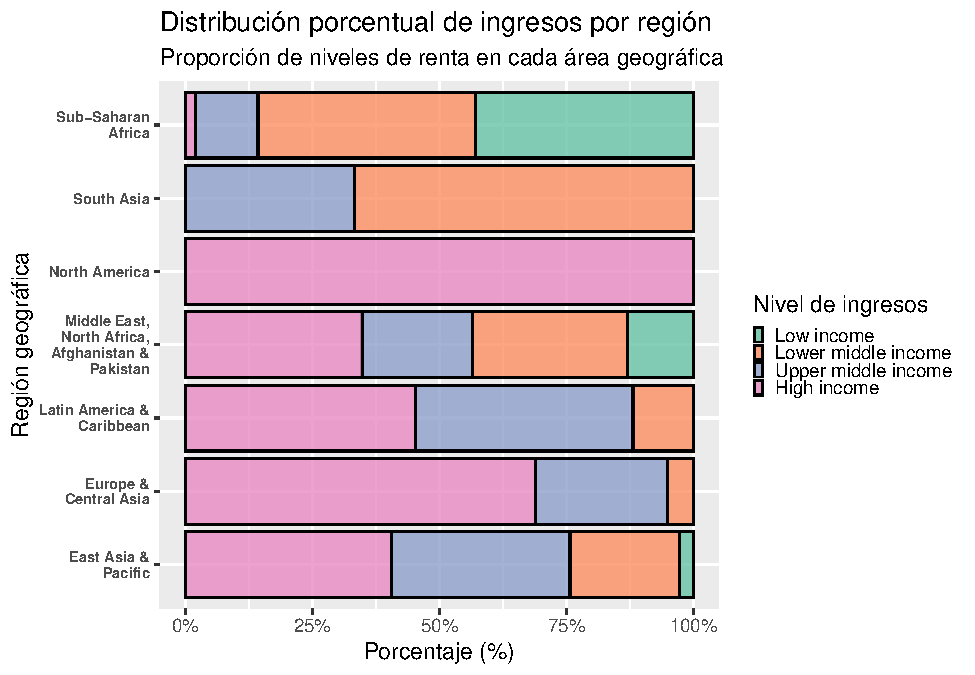
\includegraphics[keepaspectratio]{Untitled_files/figure-latex/unnamed-chunk-2-2.pdf}}

\begin{verbatim}
## Saving 6.5 x 4.5 in image
\end{verbatim}

\begin{verbatim}
## 
##  Pearson's Chi-squared test with simulated p-value (based on 10000
##  replicates)
## 
## data:  t_contingencia
## X-squared = 128.8, df = NA, p-value = 9.999e-05
\end{verbatim}

\pandocbounded{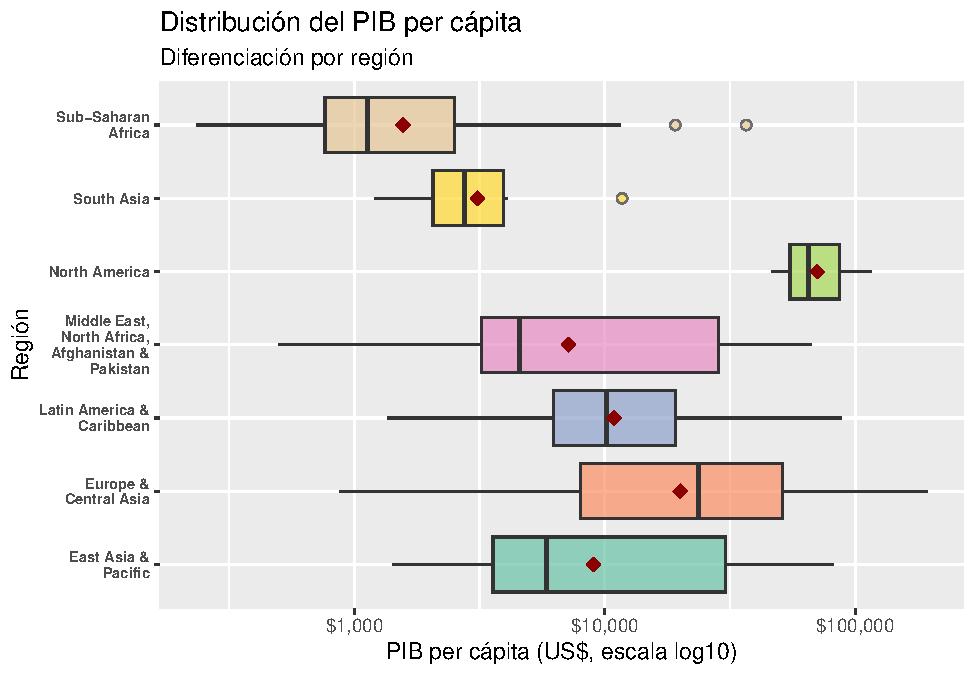
\includegraphics[keepaspectratio]{Untitled_files/figure-latex/unnamed-chunk-2-3.pdf}}

\begin{verbatim}
## Saving 6.5 x 4.5 in image
\end{verbatim}

\pandocbounded{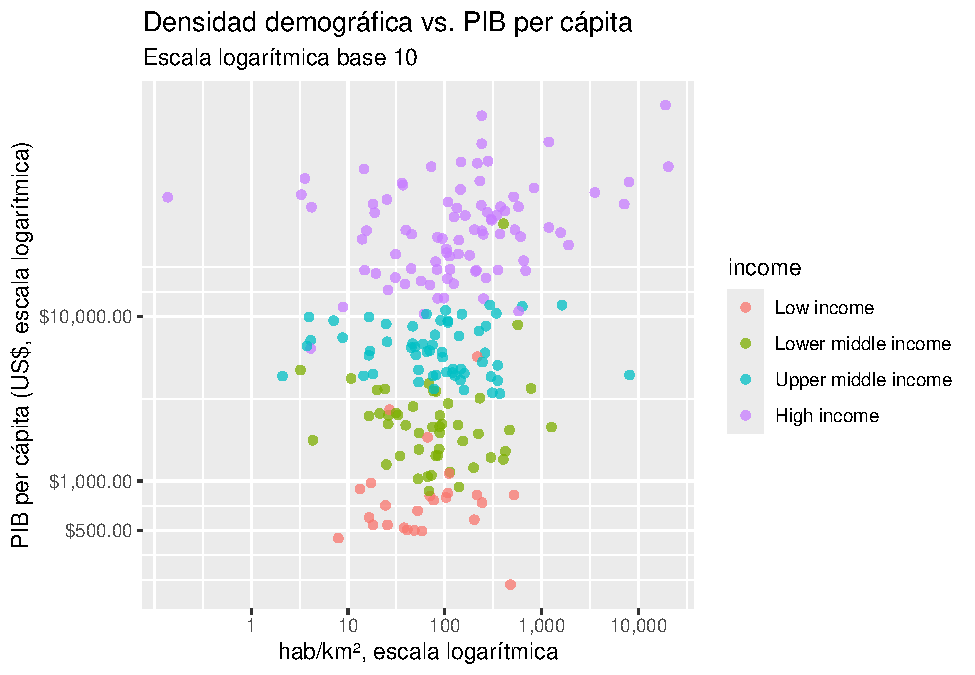
\includegraphics[keepaspectratio]{Untitled_files/figure-latex/unnamed-chunk-2-4.pdf}}

\begin{verbatim}
## Saving 6.5 x 4.5 in image
\end{verbatim}

\subsection{Bloque 2. Inversión en salud y
defensa.}\label{bloque-2.-inversiuxf3n-en-salud-y-defensa.}

El objetivo es analizar qué porcentaje del PIB por cápita se destina a
recursos sanitarios y qué porcentaje se destina a propósitos militares.
Puede tratarse de un indicador de la situación sociosanitaria del país y
de su calidad de vida, además de ser un indicativo claro para estudiar
dónde ponen el foco las autoridades a la hora de ofrecer servicios a sus
ciudadanos.

\begin{Shaded}
\begin{Highlighting}[]
\CommentTok{\# GRÁFICAS SEPARADAS}

\CommentTok{\# 1. Relación entre el gasto en defensa, gasto en sanidad y el \textquotesingle{}income\textquotesingle{}:}

\CommentTok{\# Las variables de gasto son numéricas y la variable \textquotesingle{}income\textquotesingle{} es }
\CommentTok{\# categórica. Vamos a representar gasto vs. income mediante boxplots. }
 

\CommentTok{\#Income vs. gasto en salud}
\FunctionTok{ggplot}\NormalTok{(datos\_cohorte\_2019,}
       \FunctionTok{aes}\NormalTok{(}\AttributeTok{x =}\NormalTok{ income, }\AttributeTok{y =}\NormalTok{ gasto\_salud\_gdp,}
           \AttributeTok{fill =}\NormalTok{ income)) }\SpecialCharTok{+}
  \CommentTok{\#Boxplot:}
  \FunctionTok{geom\_boxplot}\NormalTok{(}\AttributeTok{alpha =} \FloatTok{0.7}\NormalTok{,}\AttributeTok{outlier.shape =} \DecValTok{21}\NormalTok{, }\AttributeTok{outlier.size =} \DecValTok{2}\NormalTok{) }\SpecialCharTok{+}
  \CommentTok{\#Añadimos la media:}
  \FunctionTok{stat\_summary}\NormalTok{(}\AttributeTok{fun =}\NormalTok{ mean, }\AttributeTok{geom =} \StringTok{\textquotesingle{}point\textquotesingle{}}\NormalTok{, }
               \AttributeTok{shape =} \DecValTok{18}\NormalTok{,}\AttributeTok{size =} \DecValTok{3}\NormalTok{,}\AttributeTok{color =} \StringTok{\textquotesingle{}darkred\textquotesingle{}}\NormalTok{,}\FunctionTok{aes}\NormalTok{(}\AttributeTok{group =}\NormalTok{ income)) }\SpecialCharTok{+}
  \CommentTok{\#Paleta de colores:}
  \FunctionTok{scale\_fill\_brewer}\NormalTok{(}\AttributeTok{palette =} \StringTok{\textquotesingle{}Set2\textquotesingle{}}\NormalTok{) }\SpecialCharTok{+}
  \CommentTok{\#Etiquetas:}
  \FunctionTok{labs}\NormalTok{(}\AttributeTok{title =} \StringTok{\textquotesingle{}Distribución del gasto sanitario\textquotesingle{}}\NormalTok{,}
       \AttributeTok{subtitle =} \StringTok{\textquotesingle{}Diferenciación por niveles de ingresos\textquotesingle{}}\NormalTok{,}
       \AttributeTok{x =} \StringTok{\textquotesingle{}Nivel de ingresos del país\textquotesingle{}}\NormalTok{,}
       \AttributeTok{y =} \StringTok{\textquotesingle{}Gasto sanitario (\% del PIB)\textquotesingle{}}\NormalTok{,}
       \AttributeTok{fill =} \StringTok{\textquotesingle{}Ingresos\textquotesingle{}}\NormalTok{) }\SpecialCharTok{+}

  \FunctionTok{theme}\NormalTok{(}\AttributeTok{axis.text.x =} \FunctionTok{element\_text}\NormalTok{(}\AttributeTok{angle =} \DecValTok{0}\NormalTok{, }\AttributeTok{hjust =} \FloatTok{0.5}\NormalTok{, }\AttributeTok{size =} \DecValTok{7}\NormalTok{, }\AttributeTok{face =} \StringTok{\textquotesingle{}bold\textquotesingle{}}\NormalTok{),}
        \AttributeTok{legend.position =} \StringTok{\textquotesingle{}none\textquotesingle{}}\NormalTok{, }
        \AttributeTok{panel.grid.minor =} \FunctionTok{element\_blank}\NormalTok{())}
\end{Highlighting}
\end{Shaded}

\pandocbounded{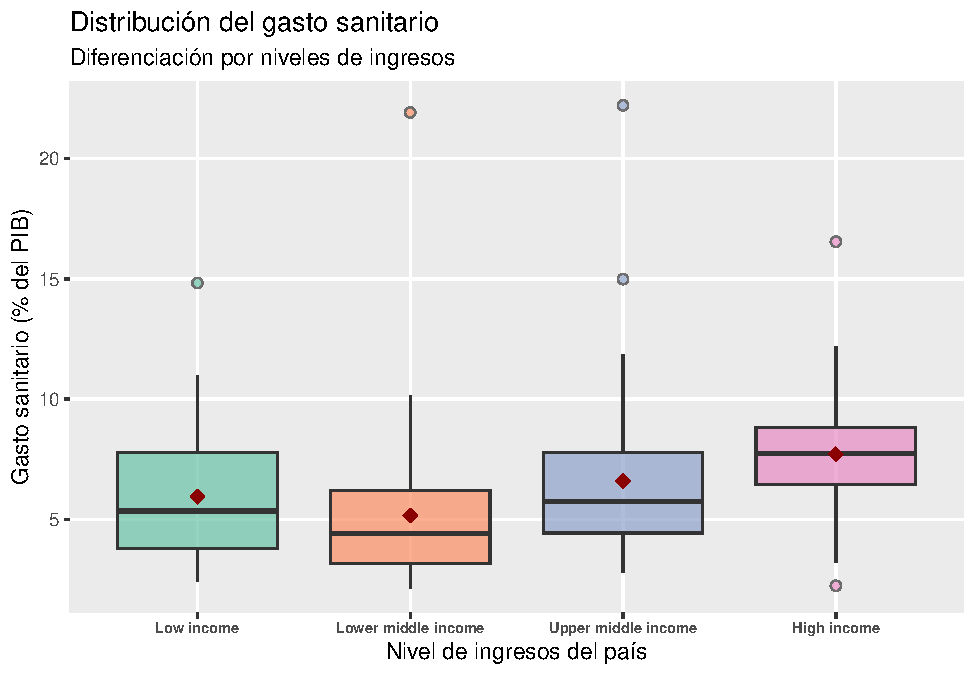
\includegraphics[keepaspectratio]{Untitled_files/figure-latex/unnamed-chunk-3-1.pdf}}

\begin{Shaded}
\begin{Highlighting}[]
\CommentTok{\# Guardamos la gráfica}
\FunctionTok{ggsave}\NormalTok{(}\StringTok{\textquotesingle{}./results/Distribucion\_gasto\_salud.pdf\textquotesingle{}}\NormalTok{)}
\end{Highlighting}
\end{Shaded}

\begin{verbatim}
## Saving 6.5 x 4.5 in image
\end{verbatim}

\begin{Shaded}
\begin{Highlighting}[]
\CommentTok{\#Income vs. gasto en defensa}
\FunctionTok{ggplot}\NormalTok{(datos\_cohorte\_2019,}
       \FunctionTok{aes}\NormalTok{(}\AttributeTok{x =}\NormalTok{ income, }\AttributeTok{y =}\NormalTok{ gasto\_defensa\_gdp,}
           \AttributeTok{fill =}\NormalTok{ income)) }\SpecialCharTok{+}
  \CommentTok{\#Boxplot:}
  \FunctionTok{geom\_boxplot}\NormalTok{(}\AttributeTok{alpha =} \FloatTok{0.7}\NormalTok{,}\AttributeTok{outlier.shape =} \DecValTok{21}\NormalTok{, }\AttributeTok{outlier.size =} \DecValTok{2}\NormalTok{) }\SpecialCharTok{+}
  \CommentTok{\#Añadimos la media:}
  \FunctionTok{stat\_summary}\NormalTok{(}\AttributeTok{fun =}\NormalTok{ mean, }\AttributeTok{geom =} \StringTok{\textquotesingle{}point\textquotesingle{}}\NormalTok{, }
               \AttributeTok{shape =} \DecValTok{18}\NormalTok{,}\AttributeTok{size =} \DecValTok{3}\NormalTok{,}\AttributeTok{color =} \StringTok{\textquotesingle{}darkred\textquotesingle{}}\NormalTok{,}\FunctionTok{aes}\NormalTok{(}\AttributeTok{group =}\NormalTok{ income)) }\SpecialCharTok{+}
  \CommentTok{\#Paleta de colores:}
  \FunctionTok{scale\_fill\_brewer}\NormalTok{(}\AttributeTok{palette =} \StringTok{\textquotesingle{}Set2\textquotesingle{}}\NormalTok{) }\SpecialCharTok{+}
  \CommentTok{\#Etiquetas:}
  \FunctionTok{labs}\NormalTok{(}\AttributeTok{title =} \StringTok{\textquotesingle{}Distribución del gasto en defensa\textquotesingle{}}\NormalTok{,}
       \AttributeTok{subtitle =} \StringTok{\textquotesingle{}Diferenciación por niveles de ingresos\textquotesingle{}}\NormalTok{,}
       \AttributeTok{x =} \StringTok{\textquotesingle{}Nivel de ingresos del país\textquotesingle{}}\NormalTok{,}
       \AttributeTok{y =} \StringTok{\textquotesingle{}Gasto militar (\% del PIB)\textquotesingle{}}\NormalTok{,}
       \AttributeTok{fill =} \StringTok{\textquotesingle{}Ingresos\textquotesingle{}}\NormalTok{) }\SpecialCharTok{+}

  \FunctionTok{theme}\NormalTok{(}\AttributeTok{axis.text.x =} \FunctionTok{element\_text}\NormalTok{(}\AttributeTok{angle =} \DecValTok{0}\NormalTok{, }\AttributeTok{hjust =} \FloatTok{0.5}\NormalTok{, }\AttributeTok{size =} \DecValTok{7}\NormalTok{, }\AttributeTok{face =} \StringTok{\textquotesingle{}bold\textquotesingle{}}\NormalTok{),}
        \AttributeTok{legend.position =} \StringTok{\textquotesingle{}none\textquotesingle{}}\NormalTok{, }
        \AttributeTok{panel.grid.minor =} \FunctionTok{element\_blank}\NormalTok{())}
\end{Highlighting}
\end{Shaded}

\pandocbounded{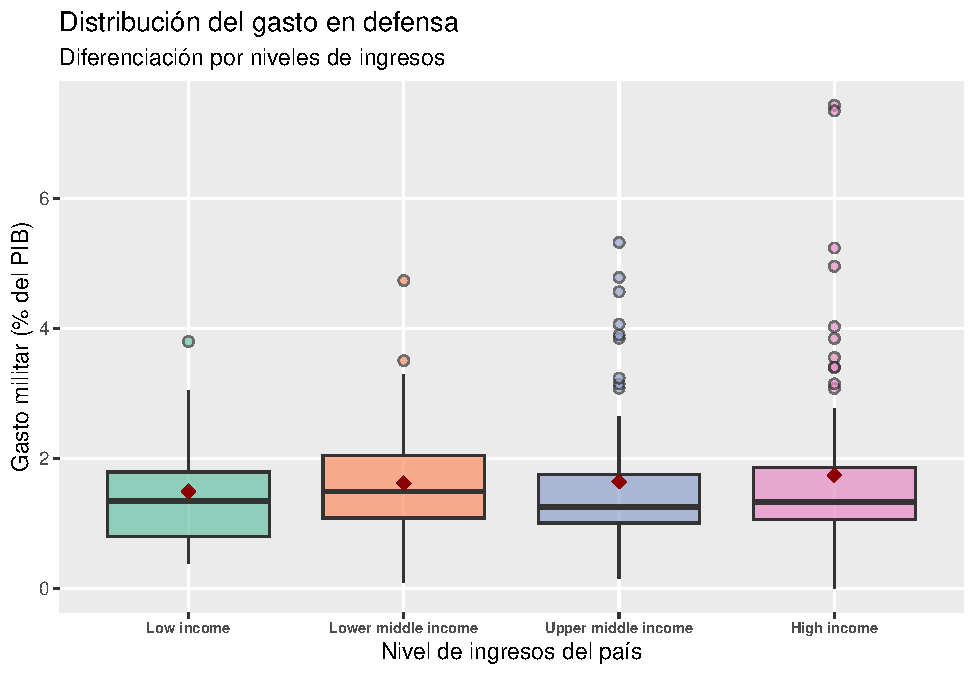
\includegraphics[keepaspectratio]{Untitled_files/figure-latex/unnamed-chunk-3-2.pdf}}

\begin{Shaded}
\begin{Highlighting}[]
\CommentTok{\# Guardamos la gráfica}
\FunctionTok{ggsave}\NormalTok{(}\StringTok{\textquotesingle{}./results/Distribucion\_gasto\_defensa.pdf\textquotesingle{}}\NormalTok{)}
\end{Highlighting}
\end{Shaded}

\begin{verbatim}
## Saving 6.5 x 4.5 in image
\end{verbatim}

\begin{Shaded}
\begin{Highlighting}[]
\CommentTok{\# 2. Relación entre el gasto en defensa, gasto en sanidad y la región:}

\CommentTok{\# Región vs. gasto sanitario}
\FunctionTok{ggplot}\NormalTok{(datos\_cohorte\_2019, }\FunctionTok{aes}\NormalTok{(}\AttributeTok{x =} \FunctionTok{str\_wrap}\NormalTok{(region, }\AttributeTok{width=}\DecValTok{15}\NormalTok{), }\AttributeTok{y =}\NormalTok{ gasto\_salud\_gdp, }
                               \AttributeTok{fill =}\NormalTok{ region)) }\SpecialCharTok{+}
  \CommentTok{\# Boxplot:}
  \FunctionTok{geom\_boxplot}\NormalTok{(}\AttributeTok{alpha =} \FloatTok{0.7}\NormalTok{, }\AttributeTok{outlier.shape =} \DecValTok{21}\NormalTok{, }\AttributeTok{outlier.size =} \DecValTok{2}\NormalTok{) }\SpecialCharTok{+}
  \CommentTok{\# Añadimos la media:}
  \FunctionTok{stat\_summary}\NormalTok{(}\AttributeTok{fun =}\NormalTok{ mean, }\AttributeTok{geom =} \StringTok{\textquotesingle{}point\textquotesingle{}}\NormalTok{, }\AttributeTok{shape =} \DecValTok{18}\NormalTok{, }
               \AttributeTok{size =} \DecValTok{3}\NormalTok{, }\AttributeTok{color =} \StringTok{\textquotesingle{}darkred\textquotesingle{}}\NormalTok{, }\FunctionTok{aes}\NormalTok{(}\AttributeTok{group =}\NormalTok{ region)) }\SpecialCharTok{+}
  \CommentTok{\# Paleta de colores:}
  \FunctionTok{scale\_fill\_brewer}\NormalTok{(}\AttributeTok{palette =} \StringTok{\textquotesingle{}Set2\textquotesingle{}}\NormalTok{) }\SpecialCharTok{+} 
  \CommentTok{\# Etiquetas:}
  \FunctionTok{labs}\NormalTok{(}\AttributeTok{title =} \StringTok{\textquotesingle{}Distribución del gasto en salud\textquotesingle{}}\NormalTok{,}
    \AttributeTok{subtitle =} \StringTok{\textquotesingle{}Diferenciación por región\textquotesingle{}}\NormalTok{,}
    \AttributeTok{x =} \StringTok{\textquotesingle{}Región\textquotesingle{}}\NormalTok{,}
    \AttributeTok{y =} \StringTok{\textquotesingle{}Gasto en salud (\% del PIB)\textquotesingle{}}\NormalTok{,}
    \AttributeTok{fill =} \StringTok{\textquotesingle{}Región\textquotesingle{}}\NormalTok{) }\SpecialCharTok{+}
  \FunctionTok{theme}\NormalTok{(}\AttributeTok{axis.text.y =} \FunctionTok{element\_text}\NormalTok{(}\AttributeTok{size =} \DecValTok{7}\NormalTok{, }\AttributeTok{face =} \StringTok{\textquotesingle{}bold\textquotesingle{}}\NormalTok{),}
        \AttributeTok{legend.position =} \StringTok{\textquotesingle{}none\textquotesingle{}}\NormalTok{) }\SpecialCharTok{+} \FunctionTok{coord\_flip}\NormalTok{()}
\end{Highlighting}
\end{Shaded}

\pandocbounded{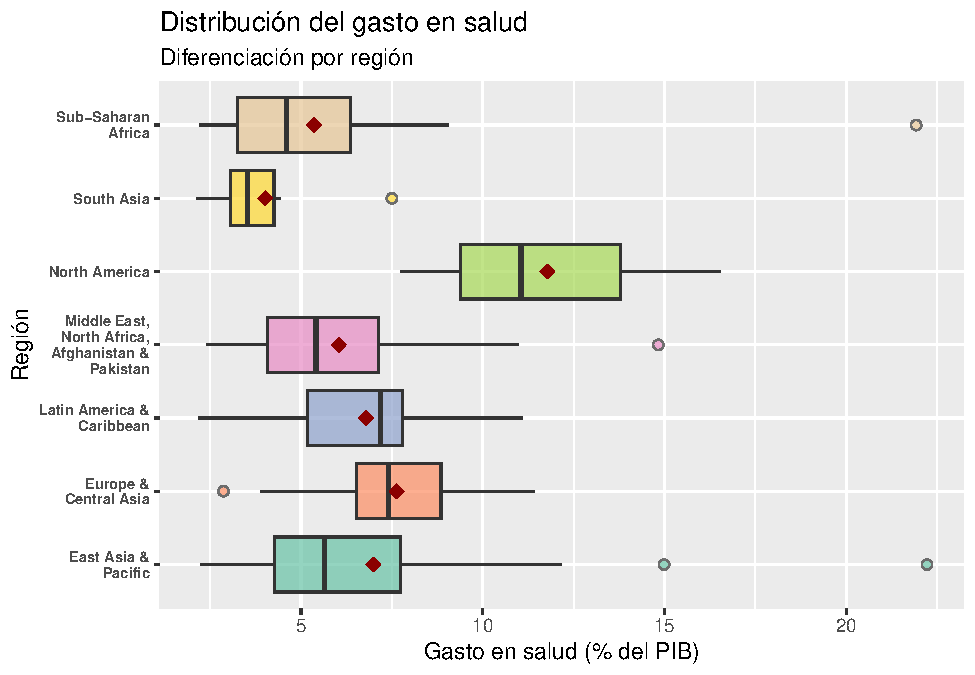
\includegraphics[keepaspectratio]{Untitled_files/figure-latex/unnamed-chunk-3-3.pdf}}

\begin{Shaded}
\begin{Highlighting}[]
\FunctionTok{ggsave}\NormalTok{(}\StringTok{\textquotesingle{}./results/Distribucion\_gasto\_salud\_region.pdf\textquotesingle{}}\NormalTok{)}
\end{Highlighting}
\end{Shaded}

\begin{verbatim}
## Saving 6.5 x 4.5 in image
\end{verbatim}

\begin{Shaded}
\begin{Highlighting}[]
\CommentTok{\# Región vs. gasto de defensa}
\FunctionTok{ggplot}\NormalTok{(datos\_cohorte\_2019, }\FunctionTok{aes}\NormalTok{(}\AttributeTok{x =} \FunctionTok{str\_wrap}\NormalTok{(region, }\AttributeTok{width=}\DecValTok{15}\NormalTok{), }\AttributeTok{y =}\NormalTok{ gasto\_defensa\_gdp, }
                               \AttributeTok{fill =}\NormalTok{ region)) }\SpecialCharTok{+}
  \CommentTok{\# Boxplot:}
  \FunctionTok{geom\_boxplot}\NormalTok{(}\AttributeTok{alpha =} \FloatTok{0.7}\NormalTok{, }\AttributeTok{outlier.shape =} \DecValTok{21}\NormalTok{, }\AttributeTok{outlier.size =} \DecValTok{2}\NormalTok{) }\SpecialCharTok{+}
  \CommentTok{\# Añadimos la media:}
  \FunctionTok{stat\_summary}\NormalTok{(}\AttributeTok{fun =}\NormalTok{ mean, }\AttributeTok{geom =} \StringTok{\textquotesingle{}point\textquotesingle{}}\NormalTok{, }\AttributeTok{shape =} \DecValTok{18}\NormalTok{, }
               \AttributeTok{size =} \DecValTok{3}\NormalTok{, }\AttributeTok{color =} \StringTok{\textquotesingle{}darkred\textquotesingle{}}\NormalTok{, }\FunctionTok{aes}\NormalTok{(}\AttributeTok{group =}\NormalTok{ region)) }\SpecialCharTok{+}
  \CommentTok{\# Paleta de colores:}
  \FunctionTok{scale\_fill\_brewer}\NormalTok{(}\AttributeTok{palette =} \StringTok{\textquotesingle{}Set2\textquotesingle{}}\NormalTok{) }\SpecialCharTok{+} 
  \CommentTok{\# Etiquetas:}
  \FunctionTok{labs}\NormalTok{(}\AttributeTok{title =} \StringTok{\textquotesingle{}Distribución del gasto en defensa\textquotesingle{}}\NormalTok{,}
    \AttributeTok{subtitle =} \StringTok{\textquotesingle{}Diferenciación por región\textquotesingle{}}\NormalTok{,}
    \AttributeTok{x =} \StringTok{\textquotesingle{}Región\textquotesingle{}}\NormalTok{,}
    \AttributeTok{y =} \StringTok{\textquotesingle{}Gasto en defensa (\% del PIB)\textquotesingle{}}\NormalTok{,}
    \AttributeTok{fill =} \StringTok{\textquotesingle{}Región\textquotesingle{}}\NormalTok{) }\SpecialCharTok{+}
  \FunctionTok{theme}\NormalTok{(}\AttributeTok{axis.text.y =} \FunctionTok{element\_text}\NormalTok{(}\AttributeTok{size =} \DecValTok{7}\NormalTok{, }\AttributeTok{face =} \StringTok{\textquotesingle{}bold\textquotesingle{}}\NormalTok{),}
        \AttributeTok{legend.position =} \StringTok{\textquotesingle{}none\textquotesingle{}}\NormalTok{) }\SpecialCharTok{+} \FunctionTok{coord\_flip}\NormalTok{()}
\end{Highlighting}
\end{Shaded}

\pandocbounded{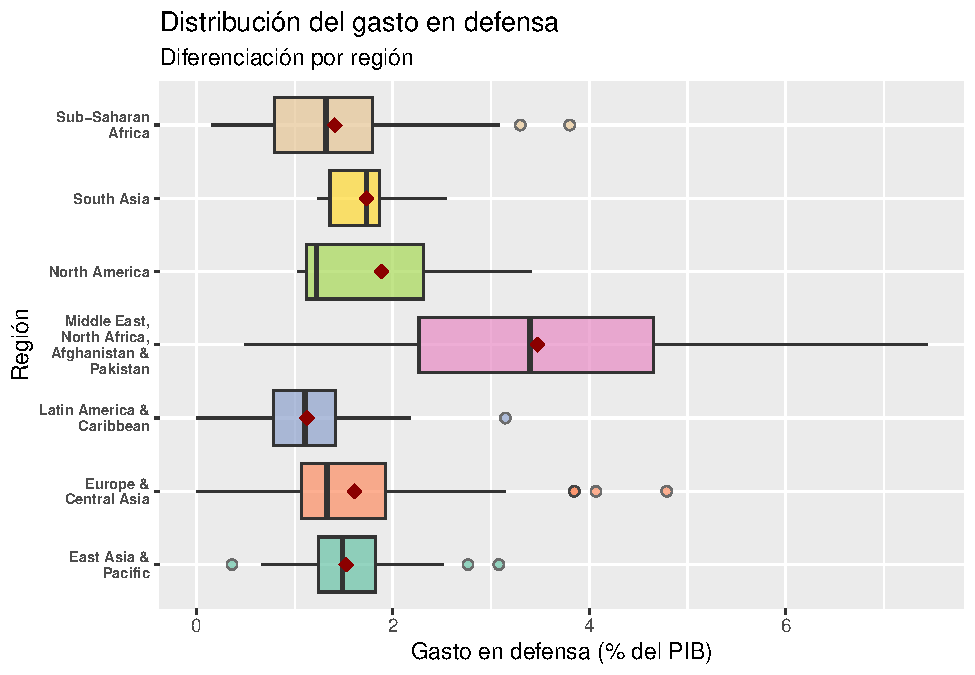
\includegraphics[keepaspectratio]{Untitled_files/figure-latex/unnamed-chunk-3-4.pdf}}

\begin{Shaded}
\begin{Highlighting}[]
\FunctionTok{ggsave}\NormalTok{(}\StringTok{\textquotesingle{}./results/Distribucion\_asto\_defensa\_region.pdf\textquotesingle{}}\NormalTok{)}
\end{Highlighting}
\end{Shaded}

\begin{verbatim}
## Saving 6.5 x 4.5 in image
\end{verbatim}

\begin{Shaded}
\begin{Highlighting}[]
\CommentTok{\# GRAFICAS JUNTAS PARA INCOME Y REGION}

\CommentTok{\# 1. Comparación entre el gasto en defensa, gasto en sanidad según \textquotesingle{}income\textquotesingle{}:}

\CommentTok{\# El objetivo de este análisis es comparar la distribución del gasto}
\CommentTok{\# sanitario y del gasto en defensa entre países pertenecientes a}
\CommentTok{\# distintos niveles de ingresos.}
\CommentTok{\#}
\CommentTok{\# Para ello, se utilizarán boxplots para poder analizar si existen diferencias en los}
\CommentTok{\# patrones de gasto según el nivel de ingresos de los países y comparar}
\CommentTok{\# la proporción del PIB que destinan a cada uno de estos ámbitos.}


\CommentTok{\# Unimos las variables de gasto sanitario y militar,}
\CommentTok{\# creando una columna que identifica el tipo de gasto}
\CommentTok{\# y otra que recoge los valores correspondientes.}

\FunctionTok{library}\NormalTok{(tidyr)}
\FunctionTok{library}\NormalTok{(dplyr)}
\NormalTok{datos\_gastos}\OtherTok{\textless{}{-}}\NormalTok{datos\_cohorte\_2019}\SpecialCharTok{\%\textgreater{}\%}\FunctionTok{select}\NormalTok{(region,income,gasto\_salud\_gdp,gasto\_defensa\_gdp)}\SpecialCharTok{\%\textgreater{}\%}
  \FunctionTok{pivot\_longer}\NormalTok{(.,}\AttributeTok{names\_to =} \StringTok{\textquotesingle{}Tipo de gasto\textquotesingle{}}\NormalTok{ ,}\AttributeTok{values\_to =} \StringTok{\textquotesingle{}Gasto (\%PIB)\textquotesingle{}}\NormalTok{ ,}\AttributeTok{cols=}\FunctionTok{c}\NormalTok{(gasto\_salud\_gdp , gasto\_defensa\_gdp) )}\SpecialCharTok{\%\textgreater{}\%}
  \FunctionTok{mutate}\NormalTok{(}\StringTok{\textasciigrave{}}\AttributeTok{Tipo de gasto}\StringTok{\textasciigrave{}}\OtherTok{=}\FunctionTok{recode}\NormalTok{(}
    \StringTok{\textasciigrave{}}\AttributeTok{Tipo de gasto}\StringTok{\textasciigrave{}}\NormalTok{ , }\AttributeTok{gasto\_salud\_gdp=}\StringTok{\textquotesingle{}Gasto en salud\textquotesingle{}}\NormalTok{, }\AttributeTok{gasto\_defensa\_gdp=}\StringTok{\textquotesingle{}Gasto en defensa\textquotesingle{}}
\NormalTok{  ))}

\FunctionTok{ggplot}\NormalTok{(datos\_gastos, }\FunctionTok{aes}\NormalTok{(}\AttributeTok{x=}\NormalTok{income,}\AttributeTok{y=}\StringTok{\textasciigrave{}}\AttributeTok{Gasto (\%PIB)}\StringTok{\textasciigrave{}}\NormalTok{,}\AttributeTok{fill=}\NormalTok{income))}\SpecialCharTok{+}
  \CommentTok{\#Boxplots:}
  \FunctionTok{geom\_boxplot}\NormalTok{(}\AttributeTok{alpha=}\FloatTok{0.7}\NormalTok{, }\AttributeTok{outlier.shape =} \DecValTok{21}\NormalTok{, }\AttributeTok{outlier.size =} \DecValTok{1}\NormalTok{)}\SpecialCharTok{+}
  \CommentTok{\#Añadimos la media:}
  \FunctionTok{stat\_summary}\NormalTok{(}\AttributeTok{fun=}\NormalTok{mean, }\AttributeTok{geom=}\StringTok{\textquotesingle{}point\textquotesingle{}}\NormalTok{,}\AttributeTok{shape=}\DecValTok{18}\NormalTok{,}\AttributeTok{size=}\DecValTok{2}\NormalTok{, }\AttributeTok{color=}\StringTok{\textquotesingle{}darkred\textquotesingle{}}\NormalTok{,}\FunctionTok{aes}\NormalTok{(}\AttributeTok{group =}\NormalTok{ income))}\SpecialCharTok{+}
  \CommentTok{\#Separamos por tipo de gasto}
  \FunctionTok{facet\_wrap}\NormalTok{(}\SpecialCharTok{\textasciitilde{}}\StringTok{\textasciigrave{}}\AttributeTok{Tipo de gasto}\StringTok{\textasciigrave{}}\NormalTok{)}\SpecialCharTok{+}
  \CommentTok{\#Paleta de colores:}
  \FunctionTok{scale\_fill\_brewer}\NormalTok{(}\AttributeTok{palette =} \StringTok{\textquotesingle{}Set2\textquotesingle{}}\NormalTok{) }\SpecialCharTok{+}
  \CommentTok{\#Etiquetas:}
  \FunctionTok{labs}\NormalTok{(}
    \AttributeTok{title =} \StringTok{\textquotesingle{}Comparación del gasto sanitario y militar\textquotesingle{}}\NormalTok{,}
    \AttributeTok{subtitle =} \StringTok{\textquotesingle{}Distribución según el nivel de ingresos\textquotesingle{}}\NormalTok{,}
    \AttributeTok{x =} \StringTok{\textquotesingle{}Nivel de ingresos del país\textquotesingle{}}\NormalTok{,}
    \AttributeTok{y =} \StringTok{\textquotesingle{}Gasto (\% del PIB)\textquotesingle{}}
\NormalTok{  ) }\SpecialCharTok{+}
  \FunctionTok{theme}\NormalTok{(}\AttributeTok{axis.text.x =} \FunctionTok{element\_text}\NormalTok{(}\AttributeTok{angle =} \DecValTok{20}\NormalTok{, }\AttributeTok{hjust =} \FloatTok{0.5}\NormalTok{, }\AttributeTok{size =} \DecValTok{5}\NormalTok{, }\AttributeTok{face =} \StringTok{\textquotesingle{}bold\textquotesingle{}}\NormalTok{),}
        \AttributeTok{legend.position =} \StringTok{\textquotesingle{}none\textquotesingle{}}\NormalTok{, }
        \AttributeTok{panel.grid.minor =} \FunctionTok{element\_blank}\NormalTok{())}
\end{Highlighting}
\end{Shaded}

\pandocbounded{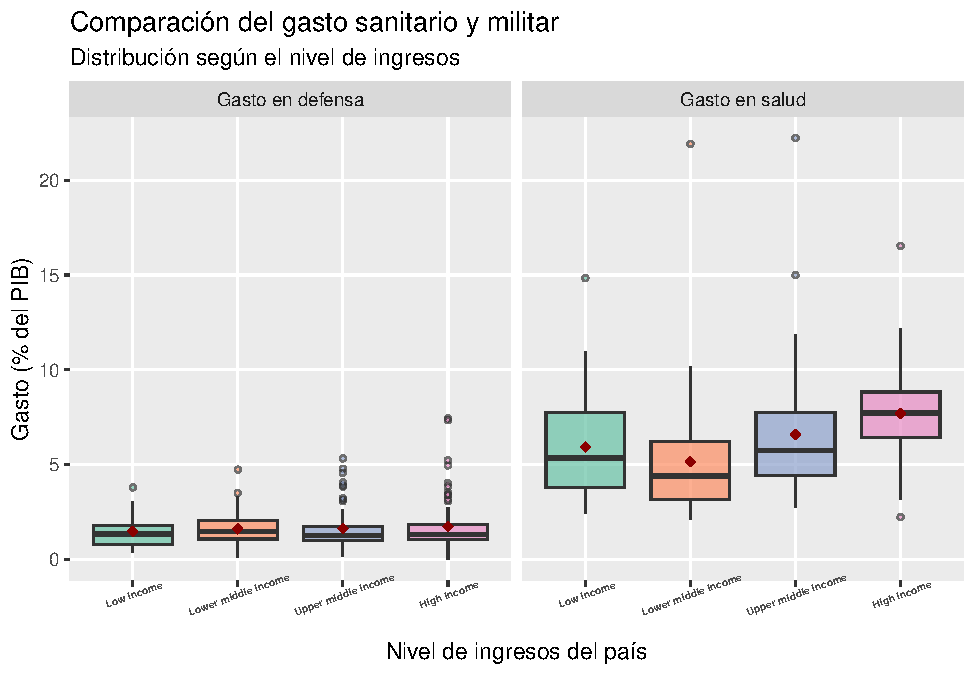
\includegraphics[keepaspectratio]{Untitled_files/figure-latex/unnamed-chunk-4-1.pdf}}

\begin{Shaded}
\begin{Highlighting}[]
\CommentTok{\# Guardamos la gráfica}
\FunctionTok{ggsave}\NormalTok{(}\StringTok{\textquotesingle{}./results/Comparacion\_gastos\_income.pdf\textquotesingle{}}\NormalTok{)}
\end{Highlighting}
\end{Shaded}

\begin{verbatim}
## Saving 6.5 x 4.5 in image
\end{verbatim}

\begin{Shaded}
\begin{Highlighting}[]
\CommentTok{\# 2. Comparación entre el gasto en defensa, gasto en sanidad según la región:}

\CommentTok{\# El objetivo de este análisis es comparar la distribución del gasto}
\CommentTok{\# sanitario y del gasto en defensa entre las distintas regiones}
\CommentTok{\# geográficas.}
\CommentTok{\#}
\CommentTok{\# Para ello, también se utilizarán boxplots para poder identificar posibles diferencias regionales}
\CommentTok{\# en los patrones de gasto y analizar qué proporción del PIB destinan}
\CommentTok{\# los países de cada región a ambos ámbitos.}


\FunctionTok{ggplot}\NormalTok{(datos\_gastos, }\FunctionTok{aes}\NormalTok{(}\AttributeTok{x=}\FunctionTok{str\_wrap}\NormalTok{(region,}\AttributeTok{width=}\DecValTok{15}\NormalTok{), }\AttributeTok{y=}\StringTok{\textasciigrave{}}\AttributeTok{Gasto (\%PIB)}\StringTok{\textasciigrave{}}\NormalTok{, }\AttributeTok{fill=}\NormalTok{region))}\SpecialCharTok{+}
  \FunctionTok{geom\_boxplot}\NormalTok{(}\AttributeTok{alpha=}\FloatTok{0.7}\NormalTok{,}\AttributeTok{outlier.shape =} \DecValTok{21}\NormalTok{,}\AttributeTok{outlier.size =} \DecValTok{1}\NormalTok{)}\SpecialCharTok{+}
  \FunctionTok{stat\_summary}\NormalTok{(}\AttributeTok{fun=}\NormalTok{mean,}\AttributeTok{geom=}\StringTok{\textquotesingle{}point\textquotesingle{}}\NormalTok{, }\AttributeTok{shape=}\DecValTok{18}\NormalTok{, }\AttributeTok{size=}\DecValTok{2}\NormalTok{, }\AttributeTok{color=}\StringTok{\textquotesingle{}darkred\textquotesingle{}}\NormalTok{, }\FunctionTok{aes}\NormalTok{(}\AttributeTok{group=}\NormalTok{region))}\SpecialCharTok{+}
  \FunctionTok{facet\_wrap}\NormalTok{(}\SpecialCharTok{\textasciitilde{}}\StringTok{\textasciigrave{}}\AttributeTok{Tipo de gasto}\StringTok{\textasciigrave{}}\NormalTok{, }\AttributeTok{ncol=}\DecValTok{1}\NormalTok{)}\SpecialCharTok{+}
  \FunctionTok{scale\_fill\_brewer}\NormalTok{(}\AttributeTok{palette=}\StringTok{\textquotesingle{}Set2\textquotesingle{}}\NormalTok{)}\SpecialCharTok{+}
  \FunctionTok{labs}\NormalTok{(}
    \AttributeTok{title =} \StringTok{\textquotesingle{}Comparación del gasto sanitario y militar\textquotesingle{}}\NormalTok{,}
    \AttributeTok{subtitle =} \StringTok{\textquotesingle{}Distribución por regiones\textquotesingle{}}\NormalTok{,}
    \AttributeTok{x =} \StringTok{\textquotesingle{}Región\textquotesingle{}}\NormalTok{,}
    \AttributeTok{y =} \StringTok{\textquotesingle{}Gasto (\% del PIB)\textquotesingle{}}
\NormalTok{  ) }\SpecialCharTok{+}
  \FunctionTok{theme}\NormalTok{(}\AttributeTok{axis.text.y =} \FunctionTok{element\_text}\NormalTok{(}\AttributeTok{angle =} \DecValTok{0}\NormalTok{, }\AttributeTok{hjust =} \FloatTok{0.5}\NormalTok{, }\AttributeTok{size =} \DecValTok{5}\NormalTok{, }\AttributeTok{face =} \StringTok{\textquotesingle{}bold\textquotesingle{}}\NormalTok{),}
        \AttributeTok{legend.position =} \StringTok{\textquotesingle{}none\textquotesingle{}}\NormalTok{, }
        \AttributeTok{panel.grid.minor =} \FunctionTok{element\_blank}\NormalTok{()) }\SpecialCharTok{+}
  
  \FunctionTok{coord\_flip}\NormalTok{()}
\end{Highlighting}
\end{Shaded}

\pandocbounded{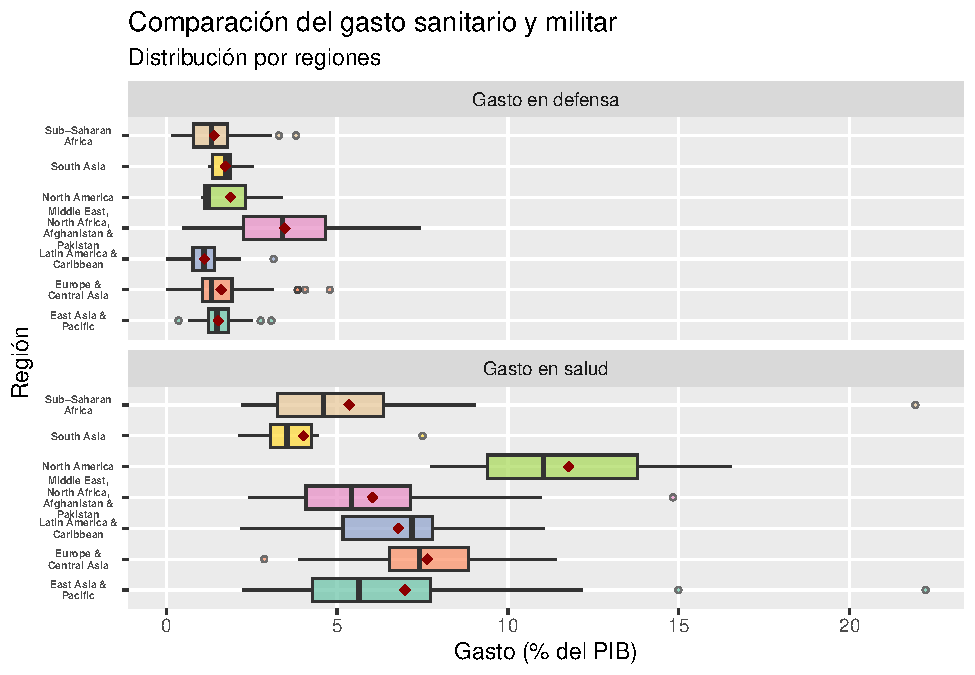
\includegraphics[keepaspectratio]{Untitled_files/figure-latex/unnamed-chunk-4-2.pdf}}

\begin{Shaded}
\begin{Highlighting}[]
\CommentTok{\# Guardamos la gráfica}
\FunctionTok{ggsave}\NormalTok{(}\StringTok{\textquotesingle{}./results/Comparacion\_gastos\_region.pdf\textquotesingle{}}\NormalTok{)}
\end{Highlighting}
\end{Shaded}

\begin{verbatim}
## Saving 6.5 x 4.5 in image
\end{verbatim}

\begin{Shaded}
\begin{Highlighting}[]
\CommentTok{\# 3. Relación entre el gasto sanitario y el gasto en defensa.}

\CommentTok{\# Representamos la relación entre ambos tipos de gastos mediante un scatter plot.}

\CommentTok{\# Vamos a tener}
\CommentTok{\# Eje X: gasto en salud (\% del PIB)}
\CommentTok{\# Eje Y: gasto en defensa (\% del PIB)}
\CommentTok{\# Nivel de ingresos por color}
 
\CommentTok{\#ggplot(datos\_cohorte\_2019, aes(x=gasto\_salud\_gdp, y=gasto\_defensa\_gdp, color=income))+}
 \CommentTok{\# geom\_point(alpha=0.75)+}
  \CommentTok{\#scale\_color\_brewer(palette=\textquotesingle{}Set2\textquotesingle{}, name=\textquotesingle{}Nivel de ingresos\textquotesingle{})+}
  \CommentTok{\#labs(}
   \CommentTok{\#title = \textquotesingle{}Relación entre el gasto sanitario y militar\textquotesingle{},}
   \CommentTok{\# subtitle = \textquotesingle{}Por nivel de ingresos\textquotesingle{},}
   \CommentTok{\# x = \textquotesingle{}Gasto en defensa (\% del PIB)\textquotesingle{},}
   \CommentTok{\# y = \textquotesingle{}Gasto sanitario (\% del PIB)\textquotesingle{},}
   \CommentTok{\# color = \textquotesingle{}Nivel de ingresos\textquotesingle{}}
 \CommentTok{\# ) + coord\_flip()}

\CommentTok{\#ggsave(\textquotesingle{}./results/Relacion\_gastos.pdf\textquotesingle{})}
\end{Highlighting}
\end{Shaded}

\subsection{Bloque 3. Necesidades
sanitarias.}\label{bloque-3.-necesidades-sanitarias.}

El objetivo de este bloque es analizar las necesidades sanitarias de los
diferentes países, estudiando cómo varían en función de su nivel de
ingresos y de su región geográfica. Para ello, se utilizarán indicadores
relacionados con la esperanza de vida, la mortalidad infantil, las
condiciones de higiene y el acceso al agua potable. Además, se estudiará
la distribución de las principales causas de mortalidad, diferenciando
entre enfermedades agudas y crónicas.

De este modo, se pretende identificar las principales desigualdades
sanitarias existentes entre países y determinar si estas están
relacionadas con su situación socioeconómica o geográfica.

\begin{Shaded}
\begin{Highlighting}[]
\CommentTok{\# BLOQUE 3. NECESIDADES SANITARIAS}

\CommentTok{\# 1. Indicadores generales de salud según income.}

\CommentTok{\# Esperanza de vida:}
\FunctionTok{ggplot}\NormalTok{(datos\_cohorte\_2019,}
       \FunctionTok{aes}\NormalTok{(}\AttributeTok{x =}\NormalTok{ income, }\AttributeTok{y =}\NormalTok{ esperanza\_vida, }\AttributeTok{fill =}\NormalTok{ income)) }\SpecialCharTok{+}
  \FunctionTok{geom\_boxplot}\NormalTok{(}\AttributeTok{alpha =} \FloatTok{0.7}\NormalTok{, }\AttributeTok{outlier.shape =} \DecValTok{21}\NormalTok{, }\AttributeTok{outlier.size =} \DecValTok{2}\NormalTok{) }\SpecialCharTok{+}
  \FunctionTok{stat\_summary}\NormalTok{(}\AttributeTok{fun =}\NormalTok{ mean, }\AttributeTok{geom =} \StringTok{\textquotesingle{}point\textquotesingle{}}\NormalTok{,}
               \AttributeTok{shape =} \DecValTok{18}\NormalTok{, }\AttributeTok{size =} \DecValTok{3}\NormalTok{, }\AttributeTok{color =} \StringTok{\textquotesingle{}darkred\textquotesingle{}}\NormalTok{) }\SpecialCharTok{+}
  \FunctionTok{scale\_fill\_brewer}\NormalTok{(}\AttributeTok{palette =} \StringTok{\textquotesingle{}Set2\textquotesingle{}}\NormalTok{) }\SpecialCharTok{+}
  \FunctionTok{labs}\NormalTok{(}
    \AttributeTok{title =} \StringTok{\textquotesingle{}Distribución de la esperanza de vida\textquotesingle{}}\NormalTok{,}
    \AttributeTok{subtitle =} \StringTok{\textquotesingle{}Diferenciación por niveles de ingresos\textquotesingle{}}\NormalTok{,}
    \AttributeTok{x =} \StringTok{\textquotesingle{}Nivel de ingresos del país\textquotesingle{}}\NormalTok{,}
    \AttributeTok{y =} \StringTok{\textquotesingle{}Esperanza de vida (años)\textquotesingle{}}
\NormalTok{  ) }\SpecialCharTok{+}
  \FunctionTok{theme}\NormalTok{(}\AttributeTok{axis.text.x =} \FunctionTok{element\_text}\NormalTok{(}\AttributeTok{size =} \DecValTok{7}\NormalTok{, }\AttributeTok{face =} \StringTok{\textquotesingle{}bold\textquotesingle{}}\NormalTok{),}
        \AttributeTok{legend.position =} \StringTok{\textquotesingle{}none\textquotesingle{}}\NormalTok{,}
        \AttributeTok{panel.grid.minor =} \FunctionTok{element\_blank}\NormalTok{())}
\end{Highlighting}
\end{Shaded}

\pandocbounded{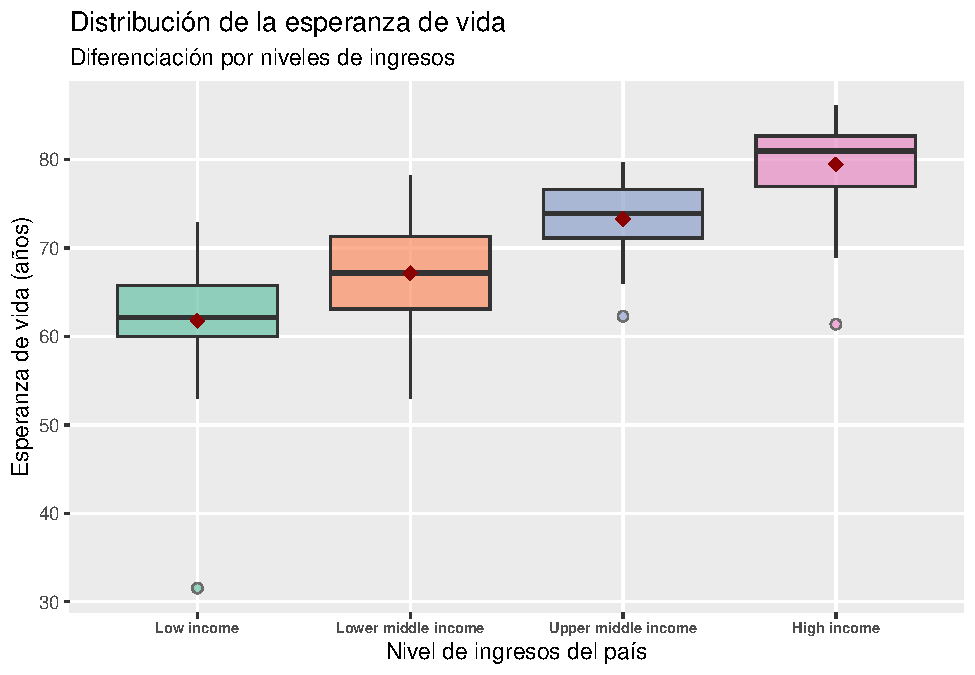
\includegraphics[keepaspectratio]{Untitled_files/figure-latex/unnamed-chunk-5-1.pdf}}

\begin{Shaded}
\begin{Highlighting}[]
\FunctionTok{ggsave}\NormalTok{(}\StringTok{\textquotesingle{}./results/Esperanza\_vida\_income.pdf\textquotesingle{}}\NormalTok{)}
\end{Highlighting}
\end{Shaded}

\begin{verbatim}
## Saving 6.5 x 4.5 in image
\end{verbatim}

\begin{Shaded}
\begin{Highlighting}[]
\CommentTok{\# Mortalidad infantil:}
\FunctionTok{ggplot}\NormalTok{(datos\_cohorte\_2019,}
       \FunctionTok{aes}\NormalTok{(}\AttributeTok{x =}\NormalTok{ income, }\AttributeTok{y =}\NormalTok{ mortalidad\_infantil, }\AttributeTok{fill =}\NormalTok{ income)) }\SpecialCharTok{+}
  \FunctionTok{geom\_boxplot}\NormalTok{(}\AttributeTok{alpha =} \FloatTok{0.7}\NormalTok{, }\AttributeTok{outlier.shape =} \DecValTok{21}\NormalTok{, }\AttributeTok{outlier.size =} \DecValTok{2}\NormalTok{) }\SpecialCharTok{+}
  \FunctionTok{stat\_summary}\NormalTok{(}\AttributeTok{fun =}\NormalTok{ mean, }\AttributeTok{geom =} \StringTok{\textquotesingle{}point\textquotesingle{}}\NormalTok{,}
               \AttributeTok{shape =} \DecValTok{18}\NormalTok{, }\AttributeTok{size =} \DecValTok{3}\NormalTok{, }\AttributeTok{color =} \StringTok{\textquotesingle{}darkred\textquotesingle{}}\NormalTok{) }\SpecialCharTok{+}
  \FunctionTok{scale\_fill\_brewer}\NormalTok{(}\AttributeTok{palette =} \StringTok{\textquotesingle{}Set2\textquotesingle{}}\NormalTok{) }\SpecialCharTok{+}
  \FunctionTok{labs}\NormalTok{(}
    \AttributeTok{title =} \StringTok{\textquotesingle{}Distribución de la mortalidad infantil\textquotesingle{}}\NormalTok{,}
    \AttributeTok{subtitle =} \StringTok{\textquotesingle{}Diferenciación por niveles de ingresos\textquotesingle{}}\NormalTok{,}
    \AttributeTok{x =} \StringTok{\textquotesingle{}Nivel de ingresos del país\textquotesingle{}}\NormalTok{,}
    \AttributeTok{y =} \StringTok{\textquotesingle{}Muertes por cada 1000 nacimientos\textquotesingle{}}
\NormalTok{  ) }\SpecialCharTok{+}
  \FunctionTok{theme}\NormalTok{(}\AttributeTok{axis.text.x =} \FunctionTok{element\_text}\NormalTok{(}\AttributeTok{size =} \DecValTok{7}\NormalTok{, }\AttributeTok{face =} \StringTok{\textquotesingle{}bold\textquotesingle{}}\NormalTok{),}
        \AttributeTok{legend.position =} \StringTok{\textquotesingle{}none\textquotesingle{}}\NormalTok{,}
        \AttributeTok{panel.grid.minor =} \FunctionTok{element\_blank}\NormalTok{())}
\end{Highlighting}
\end{Shaded}

\pandocbounded{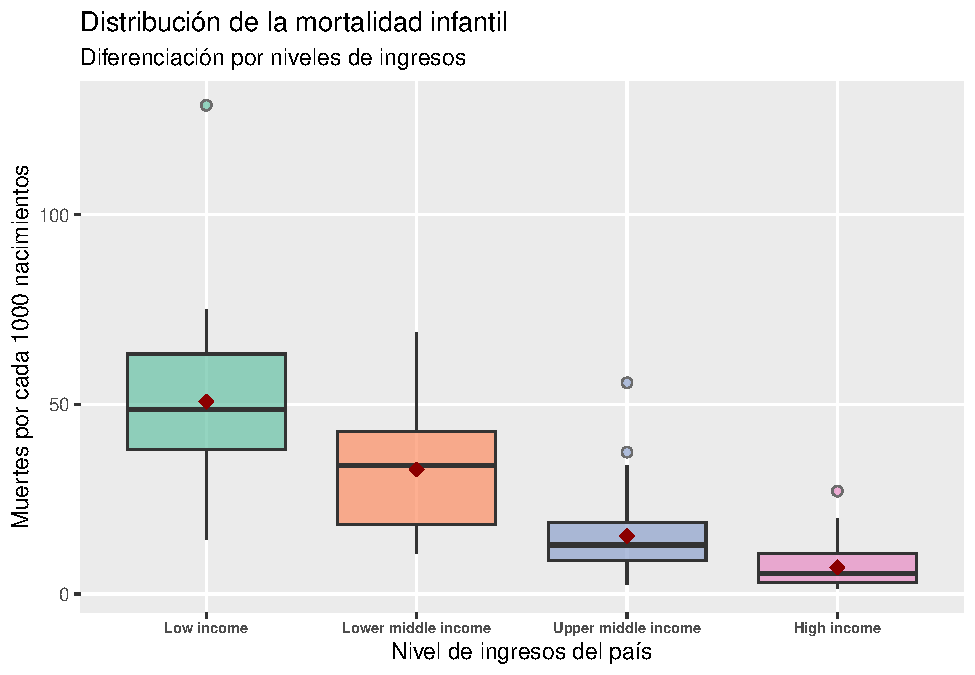
\includegraphics[keepaspectratio]{Untitled_files/figure-latex/unnamed-chunk-5-2.pdf}}

\begin{Shaded}
\begin{Highlighting}[]
\FunctionTok{ggsave}\NormalTok{(}\StringTok{\textquotesingle{}./results/Mortalidad\_infantil\_income.pdf\textquotesingle{}}\NormalTok{)}
\end{Highlighting}
\end{Shaded}

\begin{verbatim}
## Saving 6.5 x 4.5 in image
\end{verbatim}

\begin{Shaded}
\begin{Highlighting}[]
\CommentTok{\# 2. Indicadores generales de salud según región.}

\CommentTok{\# Esperanza de vida:}
\FunctionTok{ggplot}\NormalTok{(datos\_cohorte\_2019,}
       \FunctionTok{aes}\NormalTok{(}\AttributeTok{x =}\NormalTok{ stringr}\SpecialCharTok{::}\FunctionTok{str\_wrap}\NormalTok{(region, }\AttributeTok{width =} \DecValTok{15}\NormalTok{),}
           \AttributeTok{y =}\NormalTok{ esperanza\_vida, }\AttributeTok{fill =}\NormalTok{ region)) }\SpecialCharTok{+}
  \FunctionTok{geom\_boxplot}\NormalTok{(}\AttributeTok{alpha =} \FloatTok{0.7}\NormalTok{, }\AttributeTok{outlier.shape =} \DecValTok{21}\NormalTok{, }\AttributeTok{outlier.size =} \DecValTok{2}\NormalTok{) }\SpecialCharTok{+}
  \FunctionTok{stat\_summary}\NormalTok{(}\AttributeTok{fun =}\NormalTok{ mean, }\AttributeTok{geom =} \StringTok{\textquotesingle{}point\textquotesingle{}}\NormalTok{,}
               \AttributeTok{shape =} \DecValTok{18}\NormalTok{, }\AttributeTok{size =} \DecValTok{3}\NormalTok{, }\AttributeTok{color =} \StringTok{\textquotesingle{}darkred\textquotesingle{}}\NormalTok{) }\SpecialCharTok{+}
  \FunctionTok{scale\_fill\_brewer}\NormalTok{(}\AttributeTok{palette =} \StringTok{\textquotesingle{}Set2\textquotesingle{}}\NormalTok{) }\SpecialCharTok{+}
  \FunctionTok{labs}\NormalTok{(}
    \AttributeTok{title =} \StringTok{\textquotesingle{}Distribución de la esperanza de vida\textquotesingle{}}\NormalTok{,}
    \AttributeTok{subtitle =} \StringTok{\textquotesingle{}Diferenciación por región geográfica\textquotesingle{}}\NormalTok{,}
    \AttributeTok{x =} \StringTok{\textquotesingle{}Región\textquotesingle{}}\NormalTok{,}
    \AttributeTok{y =} \StringTok{\textquotesingle{}Esperanza de vida (años)\textquotesingle{}}
\NormalTok{  ) }\SpecialCharTok{+}
  \FunctionTok{theme}\NormalTok{(}\AttributeTok{axis.text.y =} \FunctionTok{element\_text}\NormalTok{(}\AttributeTok{size =} \DecValTok{7}\NormalTok{, }\AttributeTok{face =} \StringTok{\textquotesingle{}bold\textquotesingle{}}\NormalTok{),}
        \AttributeTok{legend.position =} \StringTok{\textquotesingle{}none\textquotesingle{}}\NormalTok{) }\SpecialCharTok{+}
  \FunctionTok{coord\_flip}\NormalTok{()}
\end{Highlighting}
\end{Shaded}

\pandocbounded{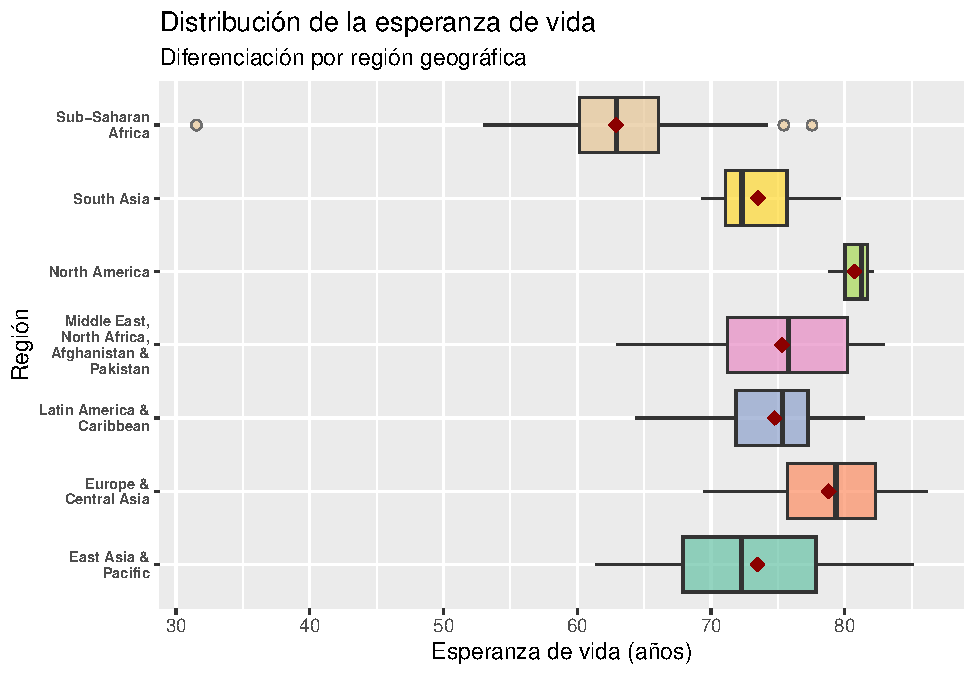
\includegraphics[keepaspectratio]{Untitled_files/figure-latex/unnamed-chunk-5-3.pdf}}

\begin{Shaded}
\begin{Highlighting}[]
\FunctionTok{ggsave}\NormalTok{(}\StringTok{\textquotesingle{}./results/Esperanza\_vida\_region.pdf\textquotesingle{}}\NormalTok{)}
\end{Highlighting}
\end{Shaded}

\begin{verbatim}
## Saving 6.5 x 4.5 in image
\end{verbatim}

\begin{Shaded}
\begin{Highlighting}[]
\CommentTok{\# Mortalidad infantil:}
\FunctionTok{ggplot}\NormalTok{(datos\_cohorte\_2019,}
       \FunctionTok{aes}\NormalTok{(}\AttributeTok{x =}\NormalTok{ stringr}\SpecialCharTok{::}\FunctionTok{str\_wrap}\NormalTok{(region, }\AttributeTok{width =} \DecValTok{15}\NormalTok{),}
           \AttributeTok{y =}\NormalTok{ mortalidad\_infantil, }\AttributeTok{fill =}\NormalTok{ region)) }\SpecialCharTok{+}
  \FunctionTok{geom\_boxplot}\NormalTok{(}\AttributeTok{alpha =} \FloatTok{0.7}\NormalTok{, }\AttributeTok{outlier.shape =} \DecValTok{21}\NormalTok{, }\AttributeTok{outlier.size =} \DecValTok{2}\NormalTok{) }\SpecialCharTok{+}
  \FunctionTok{stat\_summary}\NormalTok{(}\AttributeTok{fun =}\NormalTok{ mean, }\AttributeTok{geom =} \StringTok{\textquotesingle{}point\textquotesingle{}}\NormalTok{,}
               \AttributeTok{shape =} \DecValTok{18}\NormalTok{, }\AttributeTok{size =} \DecValTok{3}\NormalTok{, }\AttributeTok{color =} \StringTok{\textquotesingle{}darkred\textquotesingle{}}\NormalTok{) }\SpecialCharTok{+}
  \FunctionTok{scale\_fill\_brewer}\NormalTok{(}\AttributeTok{palette =} \StringTok{\textquotesingle{}Set2\textquotesingle{}}\NormalTok{) }\SpecialCharTok{+}
  \FunctionTok{labs}\NormalTok{(}
    \AttributeTok{title =} \StringTok{\textquotesingle{}Distribución de la mortalidad infantil\textquotesingle{}}\NormalTok{,}
    \AttributeTok{subtitle =} \StringTok{\textquotesingle{}Diferenciación por región geográfica\textquotesingle{}}\NormalTok{,}
    \AttributeTok{x =} \StringTok{\textquotesingle{}Región\textquotesingle{}}\NormalTok{,}
    \AttributeTok{y =} \StringTok{\textquotesingle{}Muertes por cada 1000 nacimientos\textquotesingle{}}
\NormalTok{  ) }\SpecialCharTok{+}
  \FunctionTok{theme}\NormalTok{(}\AttributeTok{axis.text.y =} \FunctionTok{element\_text}\NormalTok{(}\AttributeTok{size =} \DecValTok{7}\NormalTok{, }\AttributeTok{face =} \StringTok{\textquotesingle{}bold\textquotesingle{}}\NormalTok{),}
        \AttributeTok{legend.position =} \StringTok{\textquotesingle{}none\textquotesingle{}}\NormalTok{) }\SpecialCharTok{+}
  \FunctionTok{coord\_flip}\NormalTok{()}
\end{Highlighting}
\end{Shaded}

\pandocbounded{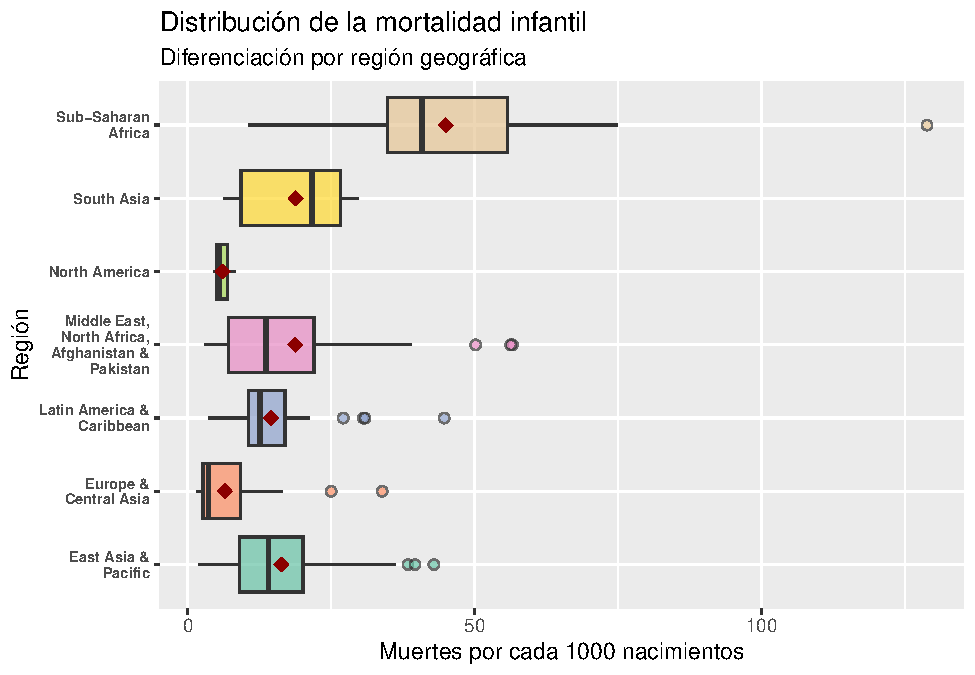
\includegraphics[keepaspectratio]{Untitled_files/figure-latex/unnamed-chunk-5-4.pdf}}

\begin{Shaded}
\begin{Highlighting}[]
\FunctionTok{ggsave}\NormalTok{(}\StringTok{\textquotesingle{}./results/Mortalidad\_infantil\_region.pdf\textquotesingle{}}\NormalTok{)}
\end{Highlighting}
\end{Shaded}

\begin{verbatim}
## Saving 6.5 x 4.5 in image
\end{verbatim}

\subsection{Correspondencia entre gasto público y
necesidades}\label{correspondencia-entre-gasto-puxfablico-y-necesidades}

Conectar los apartados anteriores para responder a la pregunta principal

\section{Discusión}\label{discusiuxf3n}

Aquí interpretaremos los resultados

\section{Conclusiones}\label{conclusiones}

Conclusiones principales del estudio

%%%%%%%%%%%%%%%%%%%%%%%%%%%%%%%%%%%%%%%%%%

\vspace{6pt}

%%%%%%%%%%%%%%%%%%%%%%%%%%%%%%%%%%%%%%%%%%
%% optional
\supplementary{The following supporting information can be downloaded
at:\\
\linksupplementary{s1}, Figure S1: title; Table S1: title; Video S1:
title.}

% Only for the journal Methods and Protocols:
% If you wish to submit a video article, please do so with any other supplementary material.
% \supplementary{The following supporting information can be downloaded at: \linksupplementary{s1}, Figure S1: title; Table S1: title; Video S1: title. A supporting video article is available at doi: link.}

%%%%%%%%%%%%%%%%%%%%%%%%%%%%%%%%%%%%%%%%%%
\authorcontributions{For research articles with several authors, a short
paragraph specifying their individual contributions must be provided.
The following statements should be used ``X.X. and Y.Y. conceive and
designed the experiments; X.X. performed the experiments; X.X. and Y.Y.
analyzed the data; W.W. contributed reagents/materials/analysis tools;
Y.Y. wrote the paper.'\,' Authorship must be limited to those who have
contributed substantially to the work reported.}

\funding{Please add:
\texttt{This\ research\ received\ no\ external\ funding\textquotesingle{}\textquotesingle{}\ or}This
research was funded by NAME OF FUNDER grant number XXX.'\,' and and
``The APC was funded by XXX'\,'. Check carefully that the details given
are accurate and use the standard spelling of funding agency names at
\url{https://search.crossref.org/funding}, any errors may affect your
future funding.}

\institutionalreview{In this section, you should add the Institutional
Review Board Statement and approval number, if relevant to your study.
You might choose to exclude this statement if the study did not require
ethical approval. Please note that the Editorial Office might ask you
for further information. Please add ``The study was conducted in
accordance with the Declaration of Helsinki, and approved by the
Institutional Review Board (or Ethics Committee) of NAME OF INSTITUTE
(protocol code XXX and date of approval).'' for studies involving
humans. OR ``The animal study protocol was approved by the Institutional
Review Board (or Ethics Committee) of NAME OF INSTITUTE (protocol code
XXX and date of approval).'' for studies involving animals. OR ``Ethical
review and approval were waived for this study due to REASON (please
provide a detailed justification).'' OR ``Not applicable'' for studies
not involving humans or animals.}

\informedconsent{Any research article describing a study involving
humans should contain this statement. Please add
\texttt{Informed\ consent\ was\ obtained\ from\ all\ subjects\ \ involved\ in\ the\ study.\textquotesingle{}\textquotesingle{}\ OR}Patient
consent was waived due to REASON (please provide a detailed
justification).'\,' OR ``Not applicable'\,' for studies not involving
humans. You might also choose to exclude this statement if the study did
not involve humans.

Written informed consent for publication must be obtained from
participating patients who can be identified (including by the patients
themselves). Please state ``Written informed consent has been obtained
from the patient(s) to publish this paper'\,' if applicable.}

\dataavailability{We encourage all authors of articles published in MDPI
journals to share their research data. In this section, please provide
details regarding where data supporting reported results can be found,
including links to publicly archived datasets analyzed or generated
during the study. Where no new data were created, or where data is
unavailable due to privacy or ethical re-strictions, a statement is
still required. Suggested Data Availability Statements are available in
section ``MDPI Research Data Policies'' at
\url{https://www.mdpi.com/ethics}.}

\acknowledgments{All sources of funding of the study should be
disclosed. Please clearly indicate grants that you have received in
support of your research work. Clearly state if you received funds for
covering the costs to publish in open access.}

\conflictsofinterest{Declare conflicts of interest or state `The authors
declare no conflict of interest.' Authors must identify and declare any
personal circumstances or interest that may be perceived as
inappropriately influencing the representation or interpretation of
reported research results. Any role of the funding sponsors in the
design of the study; in the collection, analyses or interpretation of
data in the writing of the manuscript, or in the decision to publish the
results must be declared in this section. If there is no role, please
state `The founding sponsors had no role in the design of the study; in
the collection, analyses, or interpretation of data; in the writing of
the manuscript, an in the decision to publish the results'.}

%%%%%%%%%%%%%%%%%%%%%%%%%%%%%%%%%%%%%%%%%%
%% Optional
\sampleavailability{Samples of the compounds \ldots\ldots{} are
available from the authors.}

%% Only for journal Encyclopedia

\abbreviations{Abbreviations}{
The following abbreviations are used in this manuscript:\\

\noindent
\begin{tabular}{@{}ll}
MDPI & Multidisciplinary Digital Publishing Institute \\
DOAJ & Directory of open access journals \\
TLA & Three letter acronym \\
LD & linear dichroism \\
\end{tabular}}

%%%%%%%%%%%%%%%%%%%%%%%%%%%%%%%%%%%%%%%%%%
%% Optional
\input{"appendix.tex"}
%%%%%%%%%%%%%%%%%%%%%%%%%%%%%%%%%%%%%%%%%%
\begin{adjustwidth}{-\extralength}{0cm}

%\printendnotes[custom] % Un-comment to print a list of endnotes


\reftitle{References}
\bibliography{mybibfile.bib}

% If authors have biography, please use the format below
%\section*{Short Biography of Authors}
%\bio
%{\raisebox{-0.35cm}{\includegraphics[width=3.5cm,height=5.3cm,clip,keepaspectratio]{Definitions/author1.pdf}}}
%{\textbf{Firstname Lastname} Biography of first author}
%
%\bio
%{\raisebox{-0.35cm}{\includegraphics[width=3.5cm,height=5.3cm,clip,keepaspectratio]{Definitions/author2.jpg}}}
%{\textbf{Firstname Lastname} Biography of second author}

%%%%%%%%%%%%%%%%%%%%%%%%%%%%%%%%%%%%%%%%%%
%% for journal Sci
%\reviewreports{\\
%Reviewer 1 comments and authors’ response\\
%Reviewer 2 comments and authors’ response\\
%Reviewer 3 comments and authors’ response
%}
%%%%%%%%%%%%%%%%%%%%%%%%%%%%%%%%%%%%%%%%%%
\PublishersNote{}
\end{adjustwidth}


\end{document}
